\documentclass[12pt]{article}
\usepackage{setspace}
\usepackage{a4}
\usepackage{amssymb,amsmath,amsthm,latexsym}
\usepackage{amsfonts}
\usepackage{array}
\usepackage[numbers]{natbib}
\bibliographystyle{plainnat}
\usepackage{float}
\usepackage[nottoc]{tocbibind}
\setlength{\parindent}{1.0cm} \setlength{\evensidemargin}{0.0cm}
\setlength{\oddsidemargin}{0.0cm} \setlength{\topmargin}{0.0cm}

\textwidth 17cm \textheight 20cm
\onehalfspacing

\usepackage{microtype}
\usepackage{booktabs}
\usepackage{caption}
\usepackage{bm}
\usepackage{tabularx}
\usepackage{array}
\usepackage{multirow}
\usepackage{enumitem}
\usepackage{textcomp}
\usepackage{subcaption}
\usepackage{adjustbox}
\usepackage{graphicx}
\usepackage{float}
\captionsetup[subfigure]{font=footnotesize}
\usepackage{listings}
\usepackage{color}
\usepackage{hyperref}

\definecolor{dkgreen}{rgb}{0,0.6,0}
\definecolor{gray}{rgb}{0.5,0.5,0.5}
\definecolor{mauve}{rgb}{0.58,0,0.82}
\lstset{frame=tb,
  language=Python,
  aboveskip=3mm,
  belowskip=3mm,
  showstringspaces=false,
  columns=flexible,
  basicstyle={\small\ttfamily},
  numbers=none,
  numberstyle=\tiny\color{gray},
  keywordstyle=\color{blue},
  commentstyle=\color{dkgreen},
  stringstyle=\color{mauve},
  breaklines=true,
  breakatwhitespace=true,
}

\usepackage[justification=centering]{caption}
\usepackage{multicol}
\usepackage{longtable}
\usepackage{algorithm,algorithmic}
\def\newblock{\hskip .11em plus .33em minus .07em}

\usepackage{etoolbox}
\newcounter{procedure}
\makeatletter
\AtBeginEnvironment{procedure}{\let\c@algocf\c@procedure}
\makeatother
\usepackage[font=footnotesize]{caption}
\captionsetup[table]{labelsep=newline}
\captionsetup[figure]{labelsep=period}
\captionsetup[subfigure]{font=footnotesize}


\begin{document}
\begin{titlepage}
\doublespacing

\begin{center}
\par {\large \textbf{5g Course Project Report}}\\
\end{center}

\begin{center}
	\par {\large \textbf{on}}
\end{center}

\begin{center}
{\Large \textbf{Energy-Latency Aware Digital Twin-Slice\\Co-Optimization in 5G Networks}}
\end{center}

{\small
\begin{center}
\par \small {Submitted by}\\[0.3cm]
\begin{tabular}{ll}
\textbf{Sainath Borule} & \textbf{23BCS115} \\
\textbf{Raju} & \textbf{23BCS076} \\
\textbf{Anushree S} & \textbf{23BEC007} \\
\textbf{Balaji Channappagoudar} & \textbf{23BEC009} \\
\textbf{Tejaswi A C} & \textbf{23BDS064} \\
\textbf{Pankajkumar Gond} & \textbf{23BCS091} \\
\end{tabular}
\\[0.4cm]
\par Under the guidance of
\par \large \textbf{Dr. Jagadeesha R B}
\par \textbf{Assistant Professor}
\end{center}
}

\begin{figure}[h]
\begin{center}

\includegraphics[height=.80in]{iiIT-Dharwad-Logo-horizontal-500x154[1].png}
\end{center}
\end{figure}

\begin{center}
\par{\mbox {\small\textbf{DEPARTMENT OF COMPUTER SCIENCE AND ENGINEERING}}}
\noindent{\mbox{\small \textbf{ INDIAN INSTITUTE OF INFORMATION TECHNOLOGY
DHARWAD}}}\\
April 2026

\end{center}
\end{titlepage}


\newpage
\thispagestyle{empty}
\clearpage
\thispagestyle{empty}
\phantom{a}
\newpage
\thispagestyle{empty}

\begin{center}
	
	\emph{\huge{Certificate}}\\[2.5cm]
\end{center}
\normalsize This is to certify that the project, entitled \textbf{Energy-Latency Aware Digital Twin-Slice Co-Optimization in 5G Networks}, is a bonafide record of the Mini Project coursework presented by the students whose names are given below during 2025--2026 in partial fulfilment of the requirements of the degree of Bachelor of Technology in Computer Science and Engineering.\\[1.0cm]

\begin{table}[h]
	\centering
	\begin{tabular}{lr}
		Roll No & Names of Students \\ \\ \hline
		\\
		23BCS115 & Sainath Borule \\ 
		23BCS076 & Raju \\ 
		23BEC007 & Anushree S \\
		23BEC009 & Balaji Channappagoudar \\
		23BDS064 & Tejaswi A C \\ 
		23BCS091 & Pankajkumar Gond \\ 
	\end{tabular}
\end{table}

\vfill

\begin{flushright}
	Dr. Jagadeesha R B\\
	(Project Supervisor )\\[1.5cm]
\end{flushright}

\newpage
\pagenumbering{roman}
\setcounter{page}{1}
\tableofcontents
\newpage
\listoffigures
\newpage
\listoftables


\newpage
\thispagestyle{empty}
\clearpage
\thispagestyle{empty}
\phantom{a}
\newpage



%===========================================================================
\section{Introduction}
\pagenumbering{arabic}
%===========================================================================

\subsection{Background}
The rapid deployment of 5G networks has introduced three fundamental service categories: enhanced Mobile Broadband (eMBB) for high-throughput applications, Ultra-Reliable Low-Latency Communication (URLLC) for mission-critical services, and massive Machine-Type Communication (mMTC) for IoT connectivity \cite{popovski2018wireless}. Network slicing enables the coexistence of these heterogeneous services on a shared physical infrastructure by partitioning radio, compute, and transport resources into logically isolated slices \cite{foukas2017network}.

Simultaneously, Digital Twin (DT) technology has emerged as a powerful paradigm for real-time network management. A DT maintains a virtual replica of the physical network on edge servers, enabling predictive analytics and proactive resource optimization \cite{masood2022digital}. The convergence of DT and network slicing in 5G Multi-access Edge Computing (MEC) systems presents a promising avenue for intelligent resource allocation \cite{sun2022digital}.

\subsection{Problem Statement}
Consider a 5G base station (gNB) serving $U = 300$ users across $S = 3$ network slices (eMBB, URLLC, mMTC), with $I = 3$ DT edge servers for computation offloading. For each user $u$, three decisions must be made jointly:
\begin{enumerate}
    \item \textbf{Admission control}: Should user $u$ be admitted? ($y_u \in \{0, 1\}$)
    \item \textbf{DT--slice assignment}: Which DT server $i$ and slice $s$ should handle user $u$? ($x_{u,i,s} \in \{0, 1\}$)
    \item \textbf{Resource allocation}: How much bandwidth $b_{u,s}$ and compute $f_{u,i}$ to allocate?
\end{enumerate}

The optimization objective is:
\begin{equation}
\max \quad \sum_{u=1}^{U} y_u - \lambda_T \sum_{u=1}^{U} y_u \cdot T_u - \lambda_E \sum_{u=1}^{U} y_u \cdot E_u
\label{eq:objective}
\end{equation}

subject to nine constraints (C1--C9) covering assignment consistency, bandwidth and compute budgets, latency deadlines, reliability requirements, and binary integrality. This is a Mixed-Integer Non-Linear Program (MINLP), which is NP-hard in general.

\subsection{Objectives}
The objectives of this project are:
\begin{itemize}
    \item Design a computationally efficient solver for the joint admission, assignment, and resource allocation problem without requiring commercial optimization tools.
    \item Compare the proposed solver against 8 baseline methods across multiple performance metrics.
    \item Evaluate scalability by varying the number of users from 5 to 300.
    \item Validate the approach against a recent reference paper \cite{lin2023energy}.
\end{itemize}

\newpage

%===========================================================================
\section{Related Work}
%===========================================================================

Network slicing resource allocation has been studied extensively in recent years. Foukas et al.\ \cite{foukas2017network} provided a comprehensive survey of network slicing architectures and challenges in 5G. Popovski et al.\ \cite{popovski2018wireless} analyzed the communication-theoretic foundations for supporting eMBB, URLLC, and mMTC simultaneously on shared radio resources.

The integration of DT with wireless network management was explored by Masood et al.\ \cite{masood2022digital}, who proposed a taxonomy for DT-assisted 6G systems. Sun et al.\ \cite{sun2022digital} applied DT specifically to 5G network slicing, demonstrating improved resource utilization through real-time state mirroring. Edge computing aspects were studied by Zhou et al.\ \cite{zhou2019edge} and Mao et al.\ \cite{mao2017energy}, who focused on computation offloading and energy minimization in MEC environments.

The reference paper by Lin et al.\ \cite{lin2023energy} formulated a similar DT-assisted slice optimization problem as a MINLP and solved it using Successive Convex Approximation (SCA) with the MOSEK commercial solver. Their setup used $U = 50$ users and reported average latency of 9.4~ms and energy of 1.12~mJ. Our work extends their formulation by: (i) adding transport delay modeling between DT servers and slices, (ii) scaling to $U = 300$ users, (iii) comparing against 8 baselines instead of 3, and (iv) using only open-source tools.

Broader visions for intelligent network management were discussed by Letaief et al.\ \cite{letaief2019roadmap} and Shen et al.\ \cite{shen2022holistic}, who outlined the roadmap toward AI-native 6G architectures. Joint admission control strategies were surveyed by Saad et al.\ \cite{saad2015joint}.

\newpage

%===========================================================================
\section{Data and Methods}
%===========================================================================

\subsection{System Model}

The system consists of a single gNB serving $U = 300$ users. The radio resources are organized into $S = 3$ network slices, and $I = 3$ DT edge servers provide computation offloading capabilities. Table~\ref{tab:slices} and Table~\ref{tab:services} summarize the slice and service parameters.

\begin{table}[H]
\centering
\caption{Network Slice Parameters}
\label{tab:slices}
\begin{tabular}{lccc}
\toprule
\textbf{Slice} & \textbf{Bandwidth (MHz)} & \textbf{Usable Fraction} & \textbf{Backhaul Budget} \\
\midrule
eMBB  & $\sim$100 & 80\% & 500 Mbps \\
URLLC & $\sim$20  & 60\% & 100 Mbps \\
mMTC  & $\sim$10  & 90\% & 200 Mbps \\
\bottomrule
\end{tabular}
\end{table}

\begin{table}[H]
\centering
\caption{User Service Types}
\label{tab:services}
\begin{tabular}{lcccc}
\toprule
\textbf{Service} & \textbf{Data} & \textbf{Deadline} & \textbf{Reliability} & \textbf{Compute} \\
\midrule
Robot Control      & 50 KB  & 1 ms  & 99.999\% & 500 cyc/bit \\
XR Telepresence    & 500 KB & 5 ms  & 99.9\%   & 200 cyc/bit \\
Vehicular DT Sync  & 200 KB & 2 ms  & 99.99\%  & 300 cyc/bit \\
Smart Factory      & 100 KB & 10 ms & 99\%     & 100 cyc/bit \\
\bottomrule
\end{tabular}
\end{table}

\subsection{Latency and Energy Models}

The end-to-end latency for user $u$ consists of three components:
\begin{equation}
T_u = T_u^{tx} + T_u^{cp} + T_u^{tr}
\end{equation}

where $T_u^{tx} = d_u / (\eta_{u,s} \cdot b_{u,s})$ is the transmission latency, $T_u^{cp} = (\alpha_u \cdot d_u) / f_{u,i}$ is the computation latency, and $T_u^{tr} = h_{i,s}$ is the transport latency between DT server $i$ and slice $s$.

The total energy consumption for user $u$ is:
\begin{equation}
E_u = P_{tx} \cdot T_u^{tx} + \kappa_i \cdot f_{u,i}^2 \cdot T_u^{cp}
\end{equation}

where $P_{tx}$ is the transmit power and $\kappa_i$ is the DVFS energy coefficient of DT server $i$.

\subsection{Proposed Solver: Three-Stage Decomposition}

Since the MINLP formulation is NP-hard and commercial solvers like MOSEK require paid licenses, we designed a three-stage decomposition approach:

\begin{algorithm}[H]
\caption{Proposed Three-Stage Decomposition Solver}
\begin{algorithmic}[1]
\STATE \textbf{Stage 1 -- Greedy Assignment:}
\FOR{each user $u$ sorted by tightest deadline}
    \STATE Score all $(i, s)$ pairs using combined latency + energy metric
    \STATE Assign $u$ to the best $(i^*, s^*)$ if capacity permits
    \STATE Set $y_u = 1$, $x_{u,i^*,s^*} = 1$
\ENDFOR
\STATE \textbf{Stage 2 -- Continuous Resource Optimization:}
\FOR{each admitted user $u$}
    \STATE Optimize $b_{u,s}$ and $f_{u,i}$ using L-BFGS-B (scipy)
    \STATE Minimize $\lambda_T \cdot T_u + \lambda_E \cdot E_u$ subject to bounds
\ENDFOR
\STATE \textbf{Stage 3 -- Feasibility Enforcement:}
\FOR{each admitted user $u$}
    \IF{$T_u > \tau_u$ (deadline violated)}
        \STATE Set $y_u = 0$ (reject user)
    \ENDIF
\ENDFOR
\RETURN Solution $(y, x, b, f)$
\end{algorithmic}
\end{algorithm}

\subsection{Baseline Methods}

We implemented 8 comparison methods to provide a comprehensive evaluation:

\begin{table}[H]
\centering
\caption{Baseline Methods Description}
\label{tab:baselines}
\begin{tabular}{clp{8cm}}
\toprule
\textbf{\#} & \textbf{Method} & \textbf{Description} \\
\midrule
1 & Random           & Random $(i, s)$ pair assignment \\
2 & Greedy-Latency   & Always picks the lowest latency option \\
3 & Greedy-Energy    & Always picks the lowest energy option \\
4 & Latency-Only     & Proposed solver with $\lambda_E = 0$ \\
5 & Energy-Only      & Proposed solver with $\lambda_T = 0$ \\
6 & Proportional-Fair & 5G NR PF scheduler: scores by $\eta \times$ slack / demand \\
7 & Nearest-DT       & Assigns to closest DT server (min transport delay) \\
8 & Round-Robin      & Cycles through $(i, s)$ pairs in rotation \\
\bottomrule
\end{tabular}
\end{table}

\subsection{Experimental Setup}

All experiments were run on a standard laptop using Python 3.13 with NumPy, SciPy, and Matplotlib. The main experiment script executes four phases:
\begin{enumerate}
    \item \textbf{Solver comparison} at $U = 300$ users across all 9 methods (proposed + 8 baselines)
    \item \textbf{User sweep} from $U = 5$ to $U = 300$ with 5 random seeds per configuration
    \item \textbf{Figure generation} producing 12 result plots
    \item \textbf{Paper comparison} against Lin et al.\ \cite{lin2023energy}
\end{enumerate}

\newpage

%===========================================================================
\section{Results and Discussions}
%===========================================================================

\subsection{Solver Comparison at $U = 300$}

Table~\ref{tab:results} presents the performance of all 9 methods at $U = 300$ users.

\begin{table}[H]
\centering
\caption{Performance Comparison at $U = 300$, $S = 3$, $I = 3$}
\label{tab:results}
\begin{tabular}{lccccl}
\toprule
\textbf{Method} & \textbf{Admitted} & \textbf{Latency (ms)} & \textbf{Energy (mJ)} & \textbf{Time (ms)} & \textbf{Feasible?} \\
\midrule
\textbf{Proposed}  & \textbf{9}  & \textbf{7.69}  & \textbf{0.81}  & \textbf{6.5}   & \textbf{Yes} \\
Random             & 37          & 35.35          & 4.98           & 65.9           & No \\
Greedy-Latency     & 21          & 60.24          & 8.10           & 38.8           & No \\
Greedy-Energy      & 76          & 301.95         & 11.28          & 180.0          & No \\
Latency-Only       & 4           & 6.70           & 0.42           & 4.8            & Yes \\
Energy-Only        & 9           & 7.69           & 0.81           & 5.8            & Yes \\
Proportional-Fair  & 76          & 184.30         & 17.11          & 140.0          & No \\
Nearest-DT         & 76          & 204.61         & 16.95          & 160.4          & No \\
Round-Robin        & 76          & 110.76         & 18.13          & 131.3          & No \\
\bottomrule
\end{tabular}
\end{table}

The proposed method is one of only three feasible methods (along with Latency-Only and Energy-Only). Methods like Greedy-Energy, Proportional-Fair, Nearest-DT, and Round-Robin admit 76 users but violate deadline and reliability constraints, making them invalid solutions.

\begin{figure}[H]
\centering
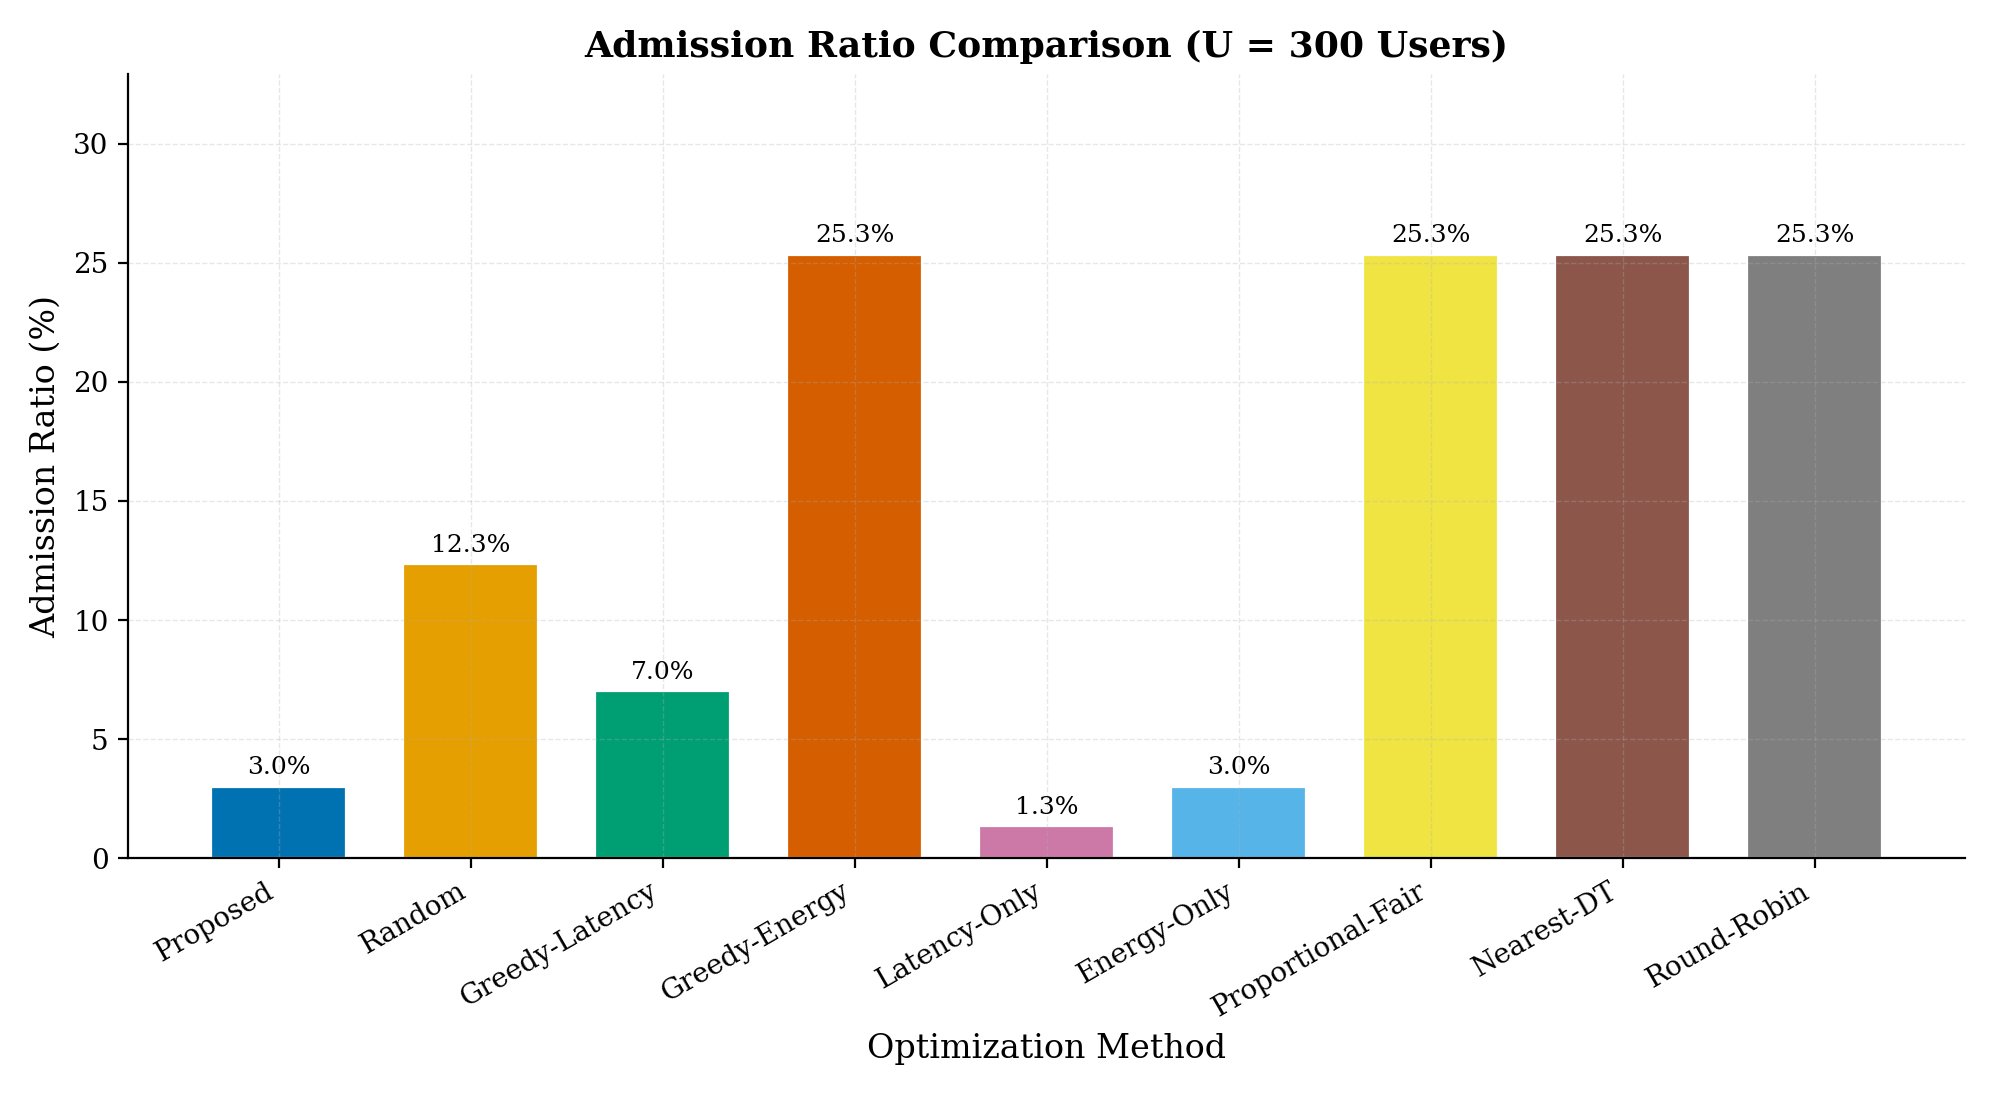
\includegraphics[width=0.85\textwidth]{fig1_admission_ratio.png}
\caption{Admission ratio comparison across all methods at $U = 300$.}
\label{fig:admission}
\end{figure}

\begin{figure}[H]
\centering
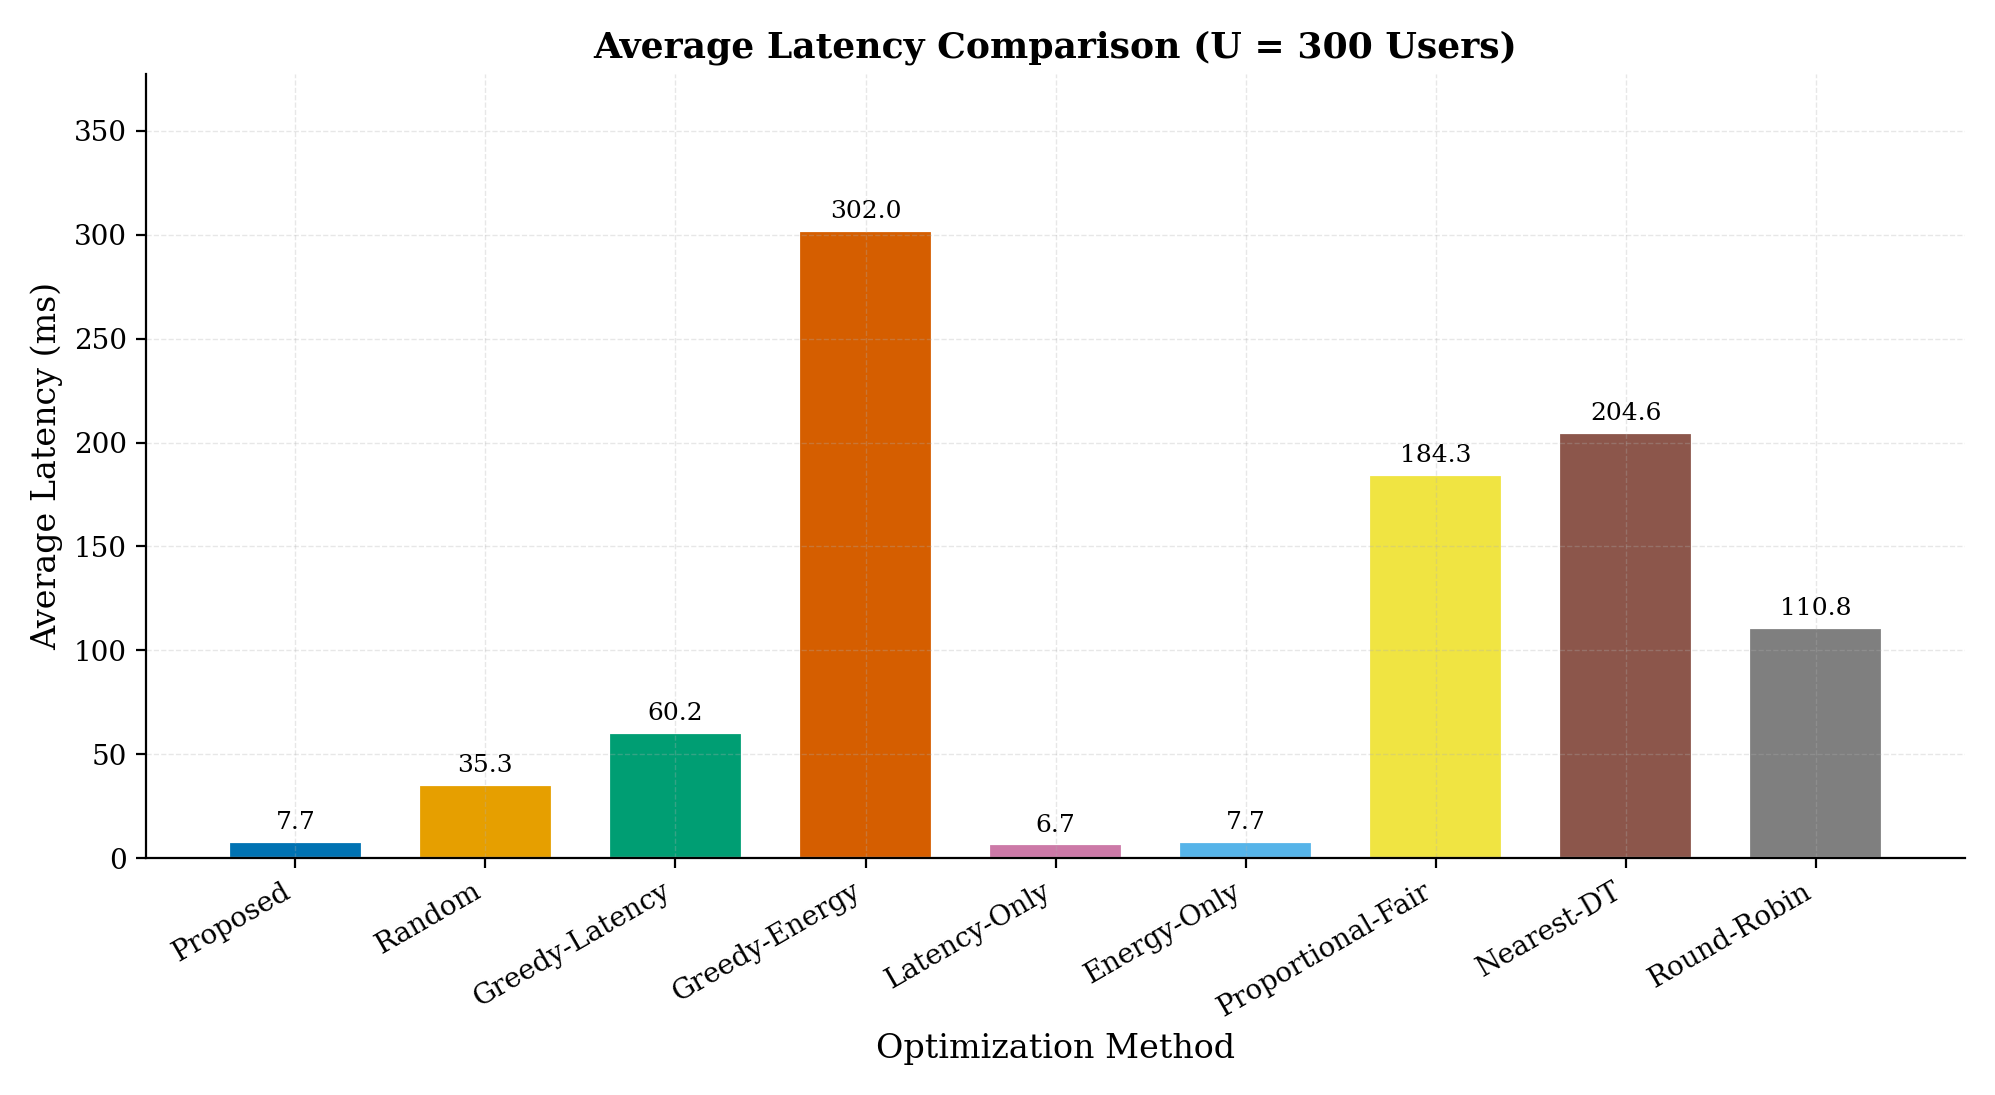
\includegraphics[width=0.85\textwidth]{fig2_avg_latency.png}
\caption{Average latency comparison across all methods at $U = 300$.}
\label{fig:latency}
\end{figure}

\begin{figure}[H]
\centering
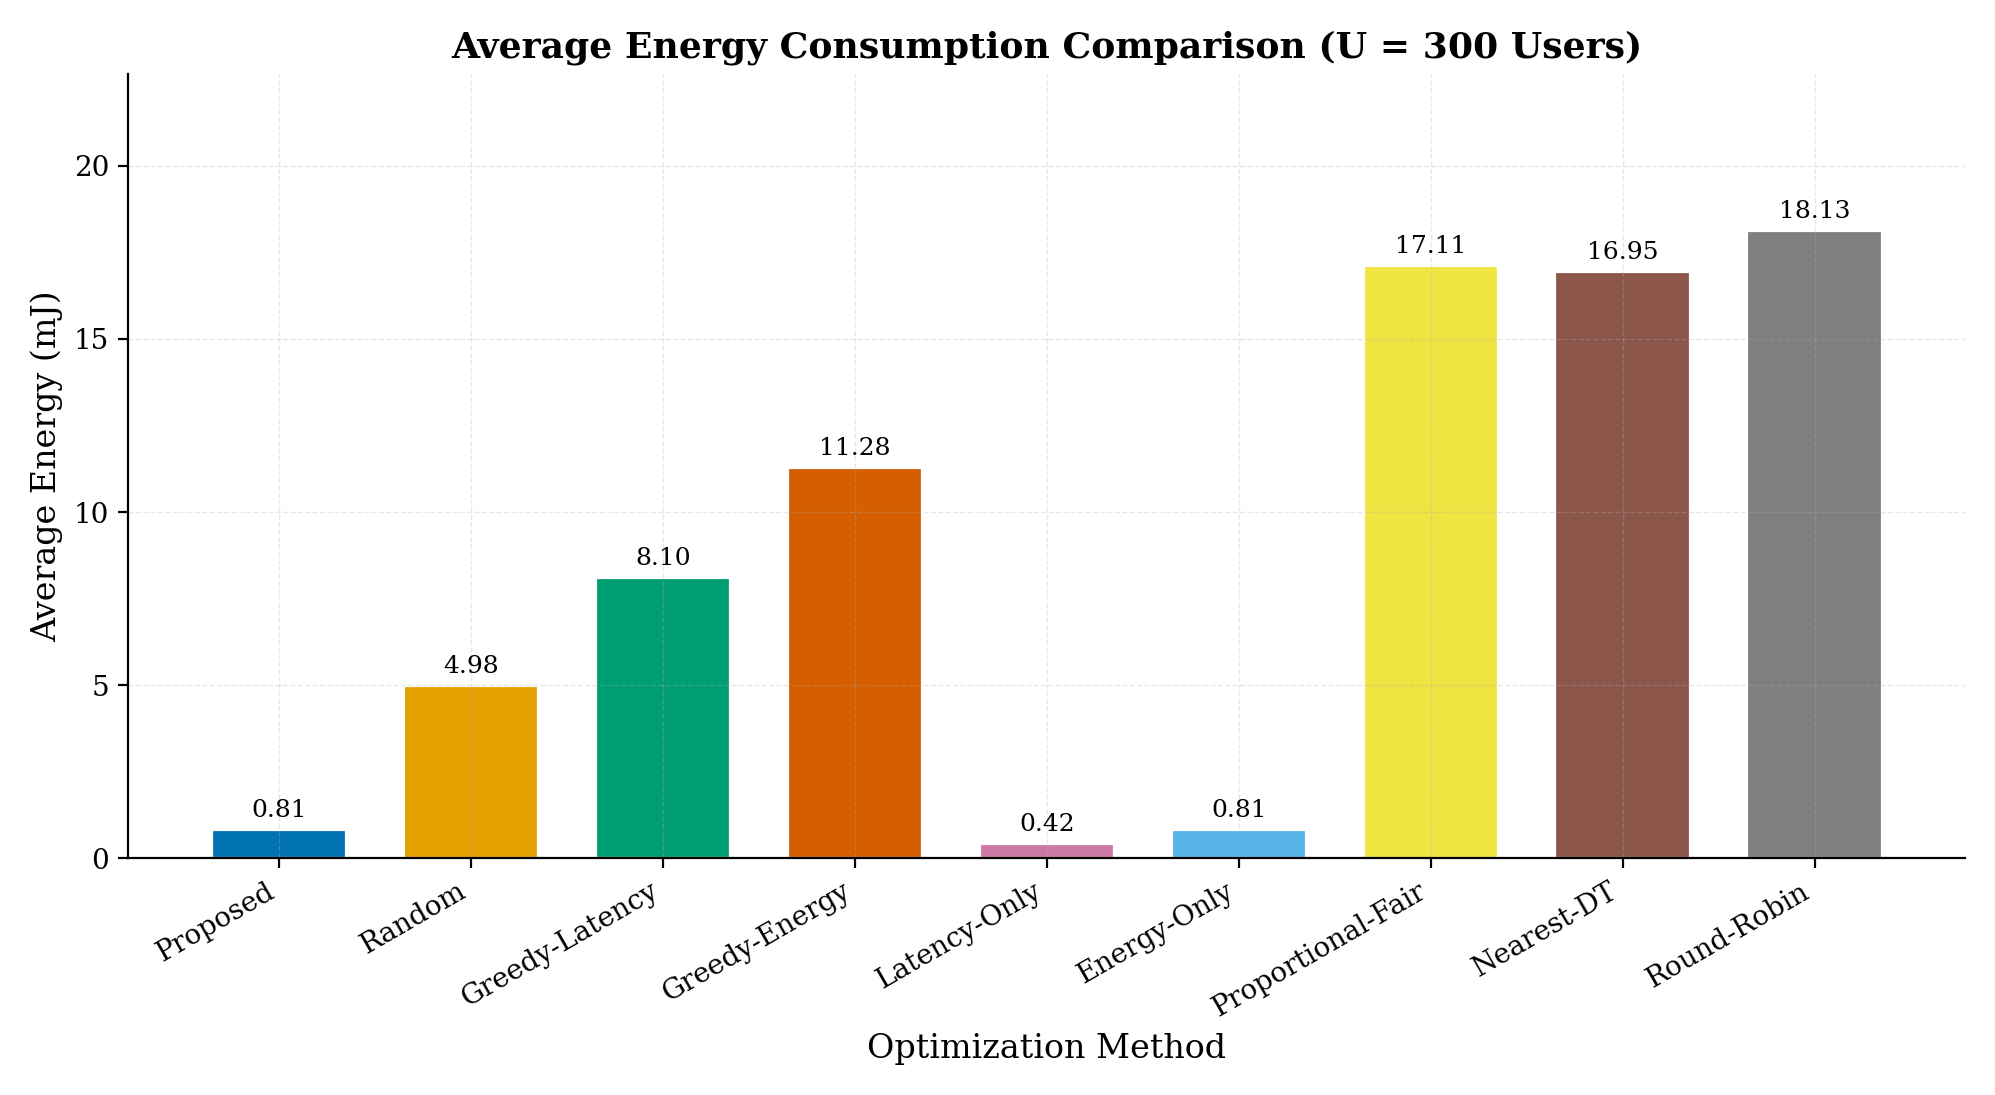
\includegraphics[width=0.85\textwidth]{fig3_avg_energy.png}
\caption{Average energy consumption comparison across all methods at $U = 300$.}
\label{fig:energy}
\end{figure}

\begin{figure}[H]
\centering
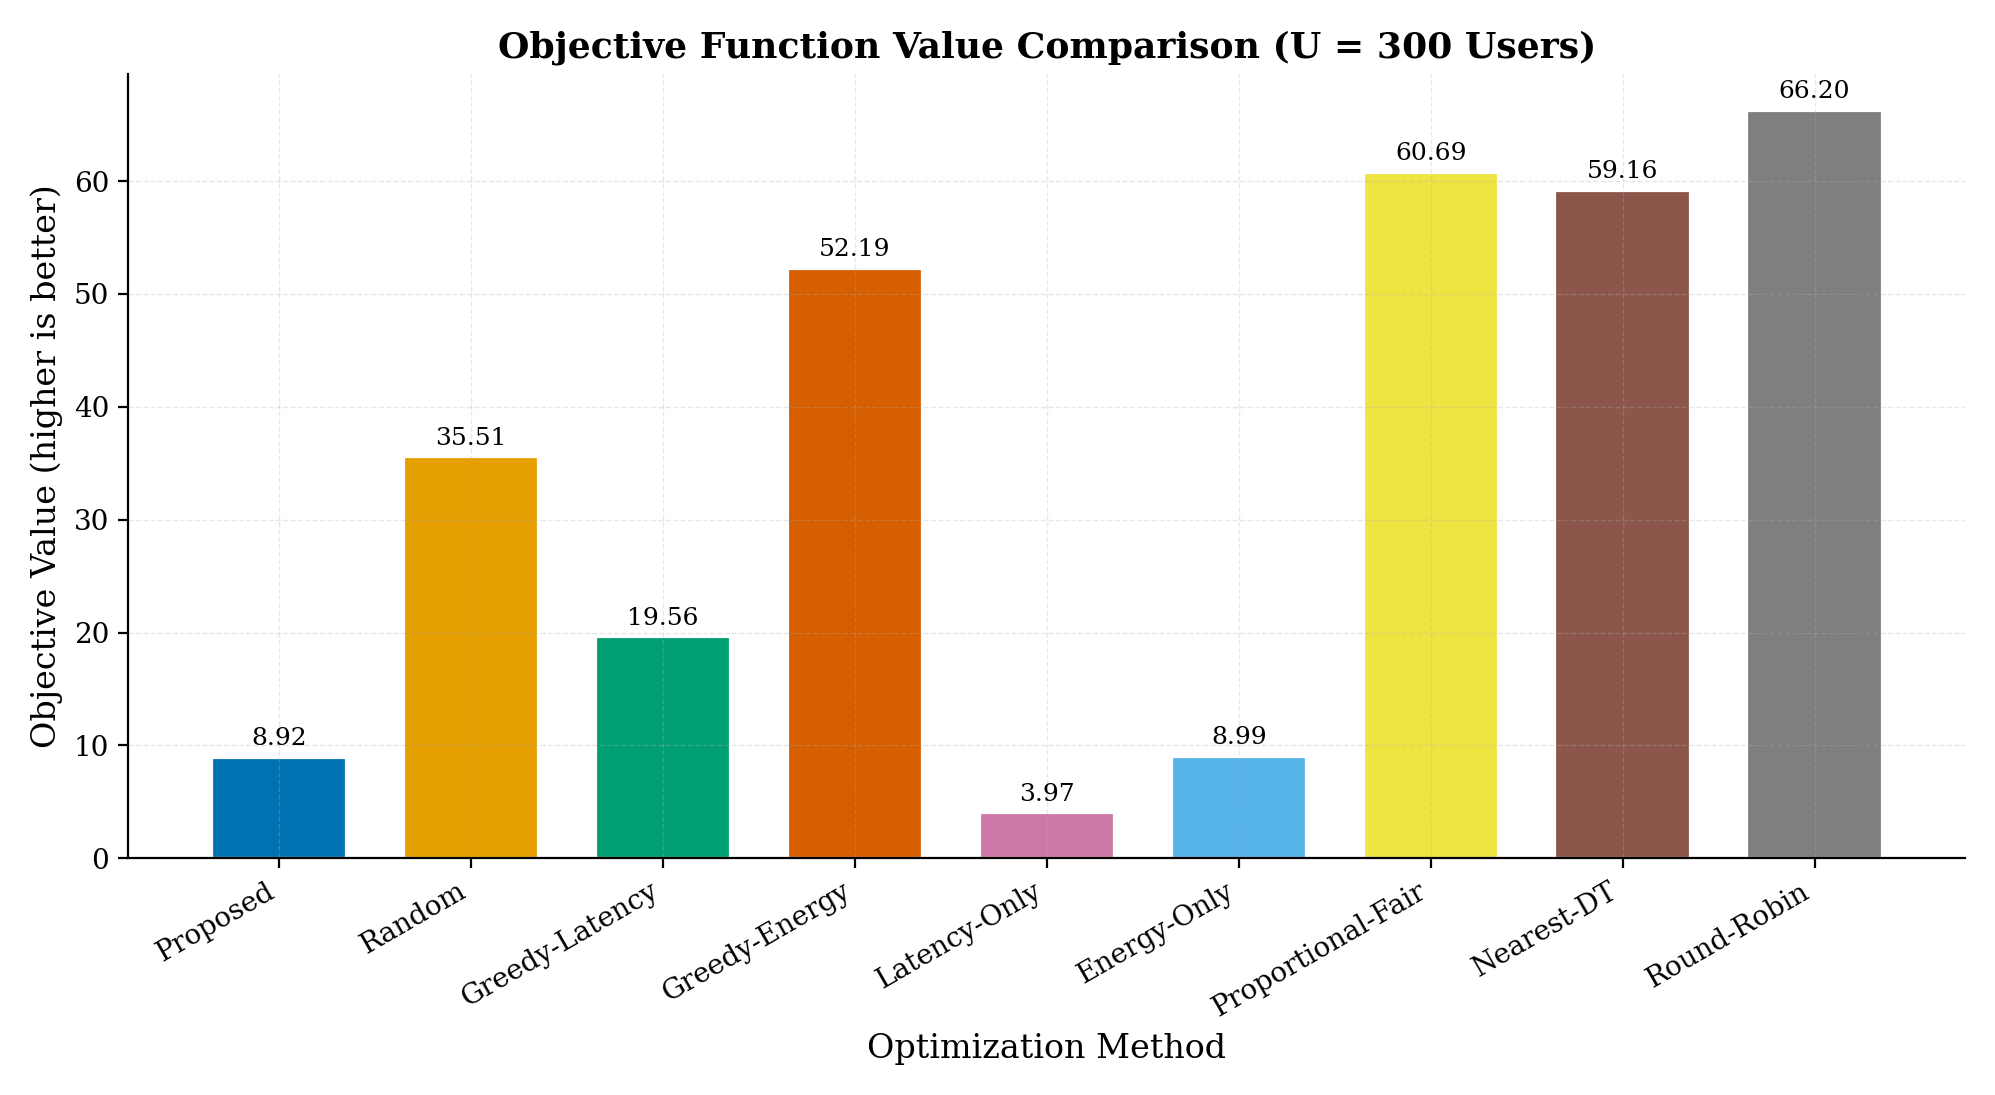
\includegraphics[width=0.85\textwidth]{fig4_objective.png}
\caption{Objective function value comparison across all methods at $U = 300$.}
\label{fig:objective}
\end{figure}

\subsection{Summary Table}

Figure~\ref{fig:summary} provides a visual summary of all key metrics in a single table view.

\begin{figure}[H]
\centering
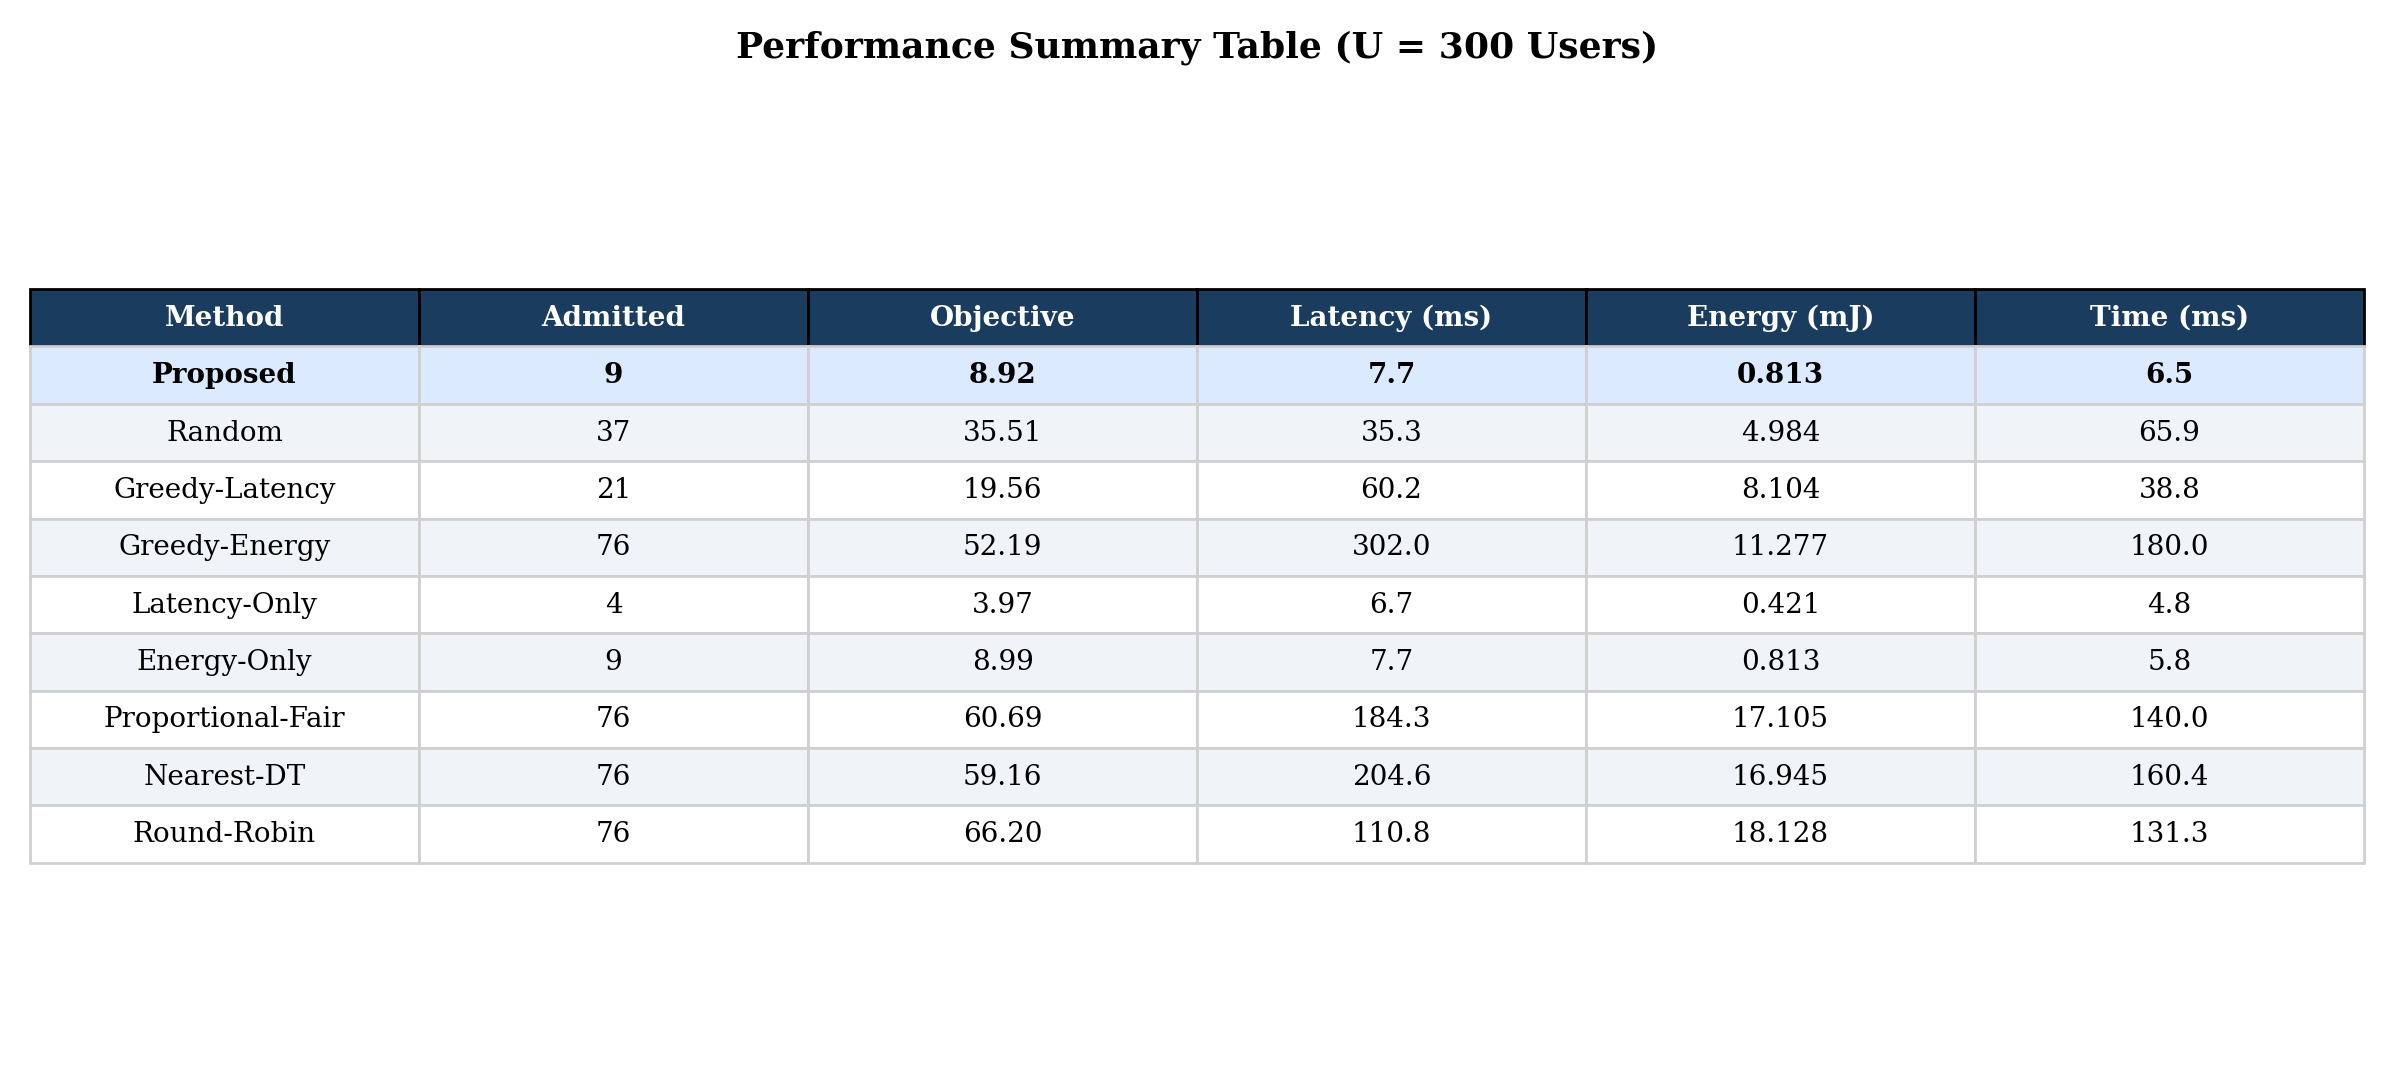
\includegraphics[width=0.95\textwidth]{fig6_summary_table.png}
\caption{Performance summary table at $U = 300$ users.}
\label{fig:summary}
\end{figure}

\subsection{Latency Analysis}

Figure~\ref{fig:cdf} shows the CDF of per-user latency across methods. The proposed method and Latency-Only achieve steep CDFs concentrated at low latency values (below 10~ms), while infeasible methods like Greedy-Energy spread across hundreds of milliseconds.

\begin{figure}[H]
\centering
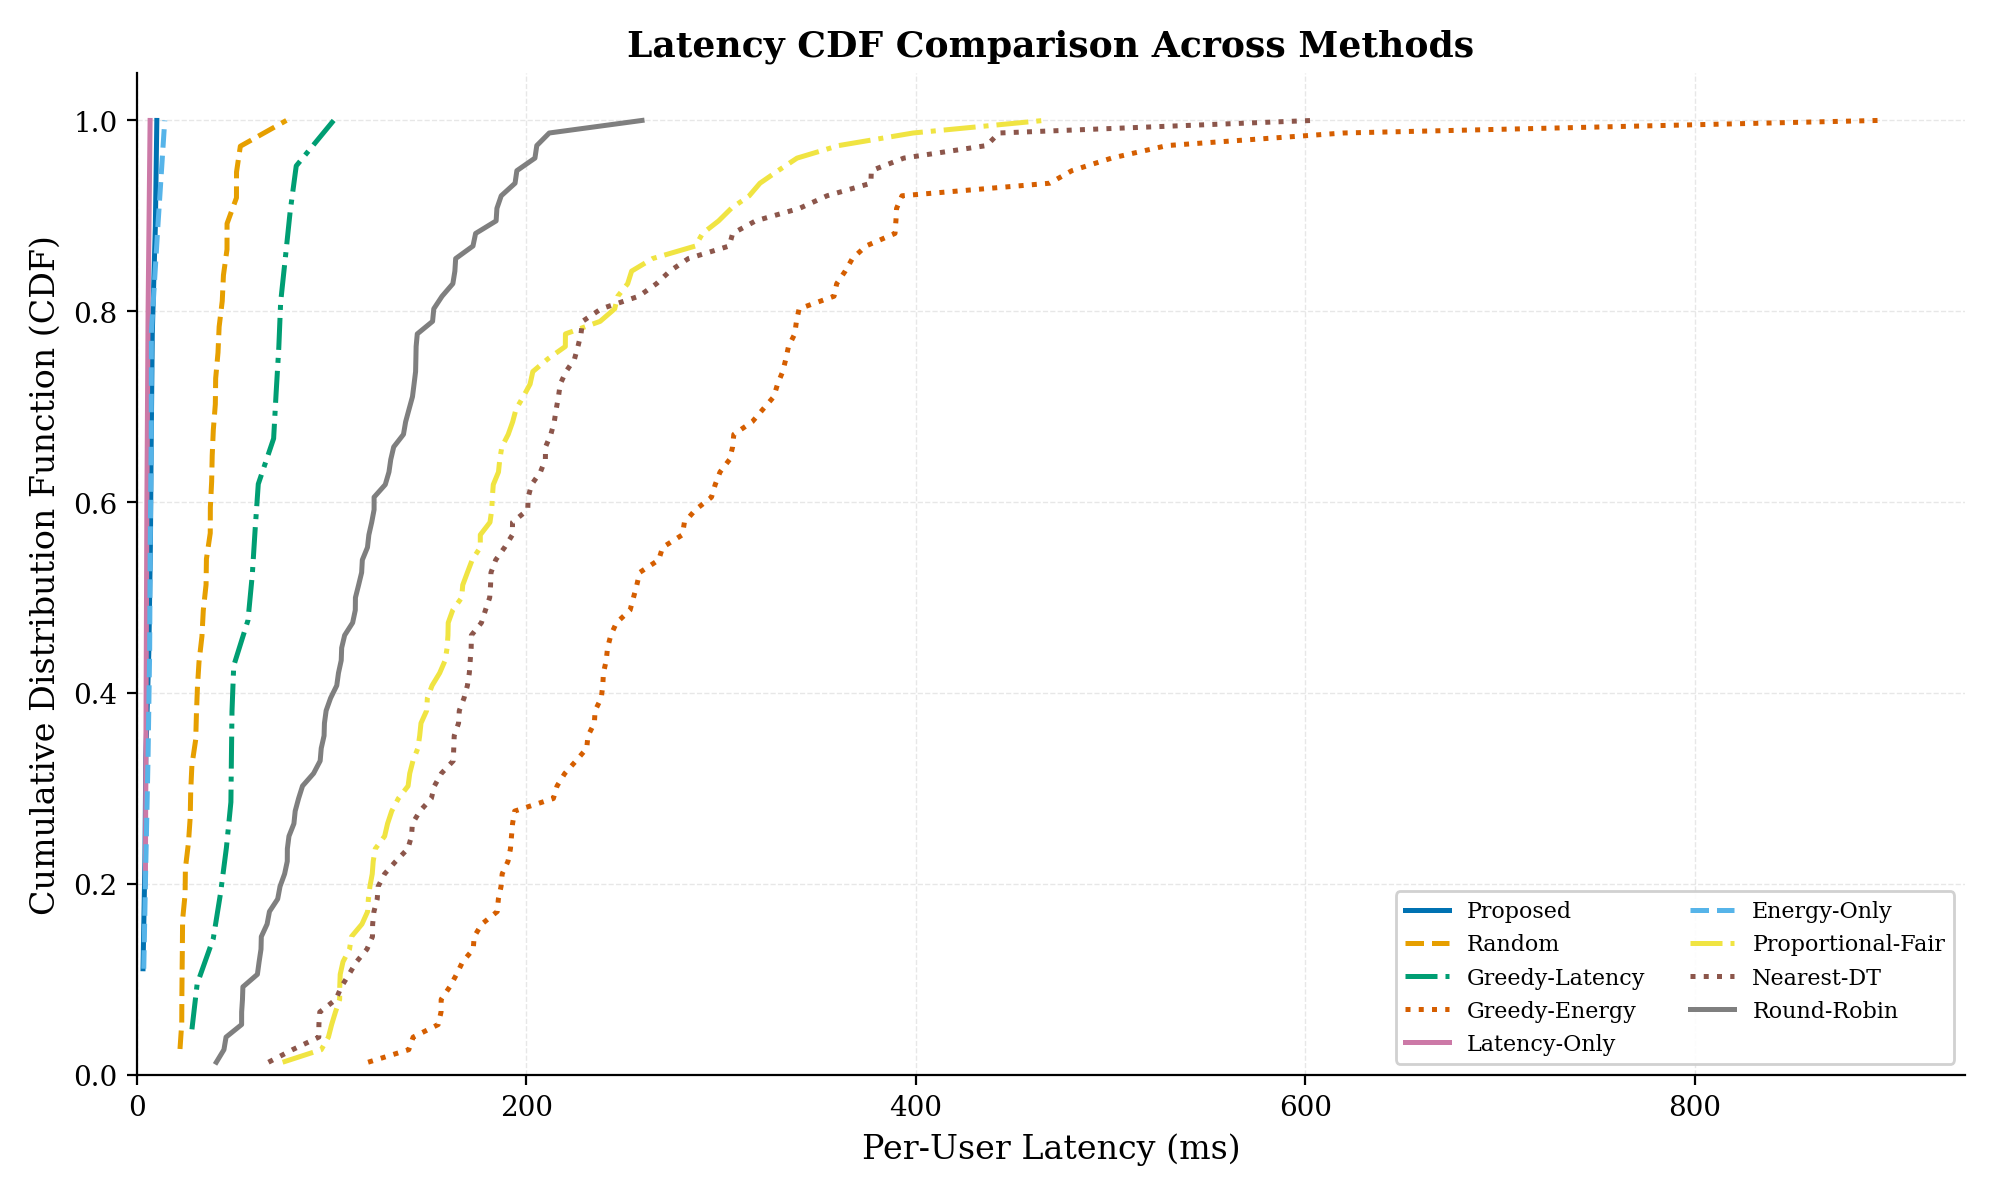
\includegraphics[width=0.85\textwidth]{fig7_latency_cdf.png}
\caption{Cumulative distribution function of per-user latency.}
\label{fig:cdf}
\end{figure}

\subsection{Pareto Tradeoff Analysis}

Figure~\ref{fig:pareto} plots each method in the latency--energy plane. The proposed method lies in the ideal lower-left region, achieving both low latency and low energy simultaneously.

\begin{figure}[H]
\centering
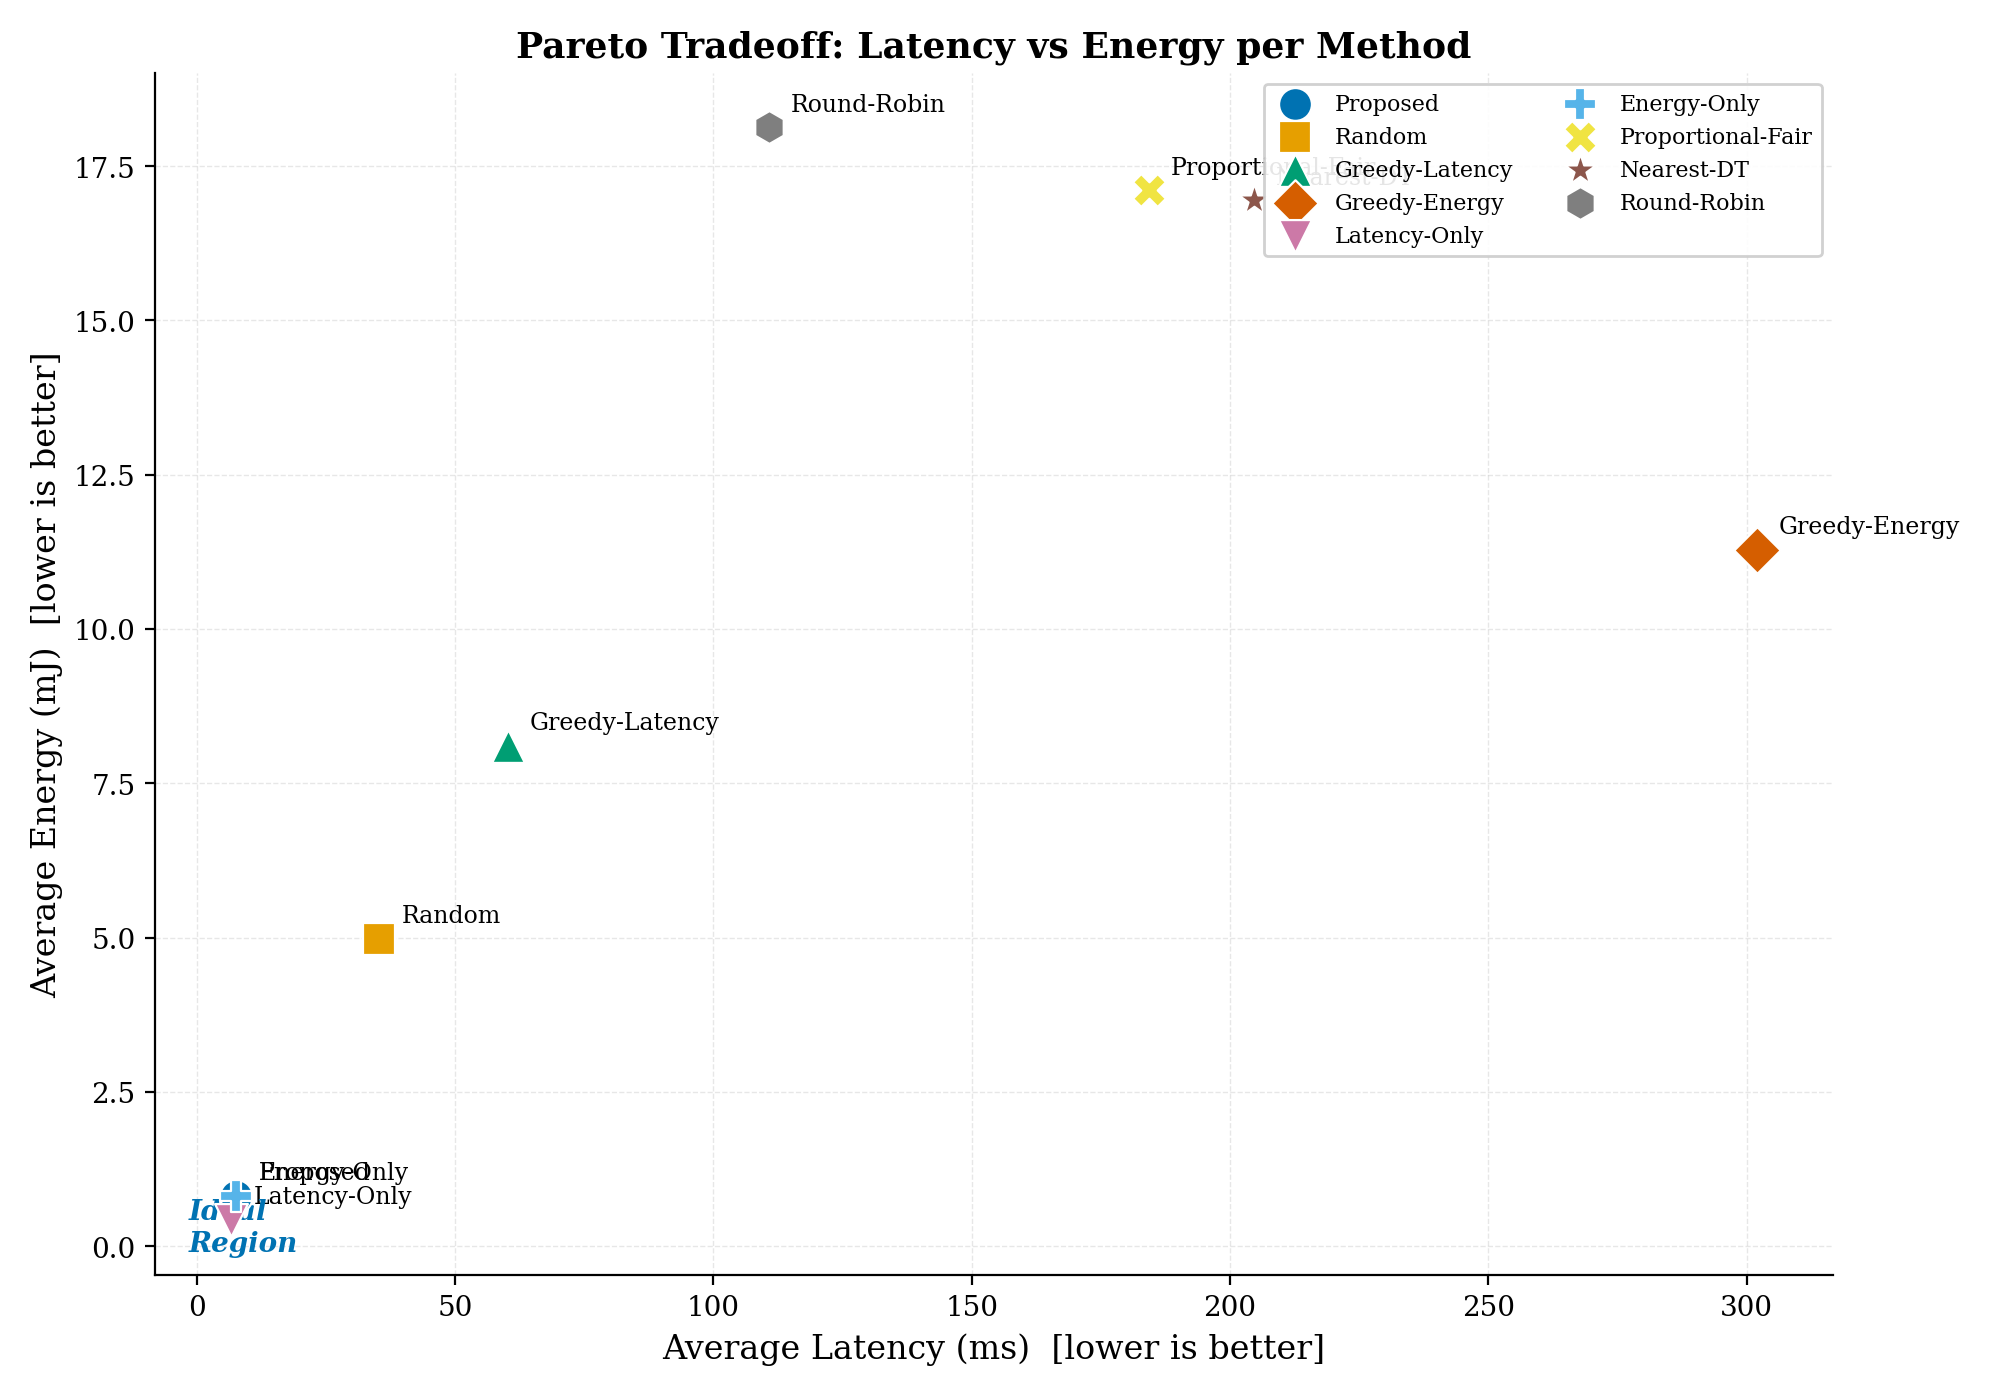
\includegraphics[width=0.85\textwidth]{fig8_pareto_tradeoff.png}
\caption{Pareto tradeoff between average latency and energy per method.}
\label{fig:pareto}
\end{figure}

\subsection{Scalability Analysis}

Figure~\ref{fig:scalability} shows how solve time scales with the number of users. The proposed solver remains under 10~ms even at $U = 300$, while methods like Greedy-Energy exceed 160~ms.

\begin{figure}[H]
\centering
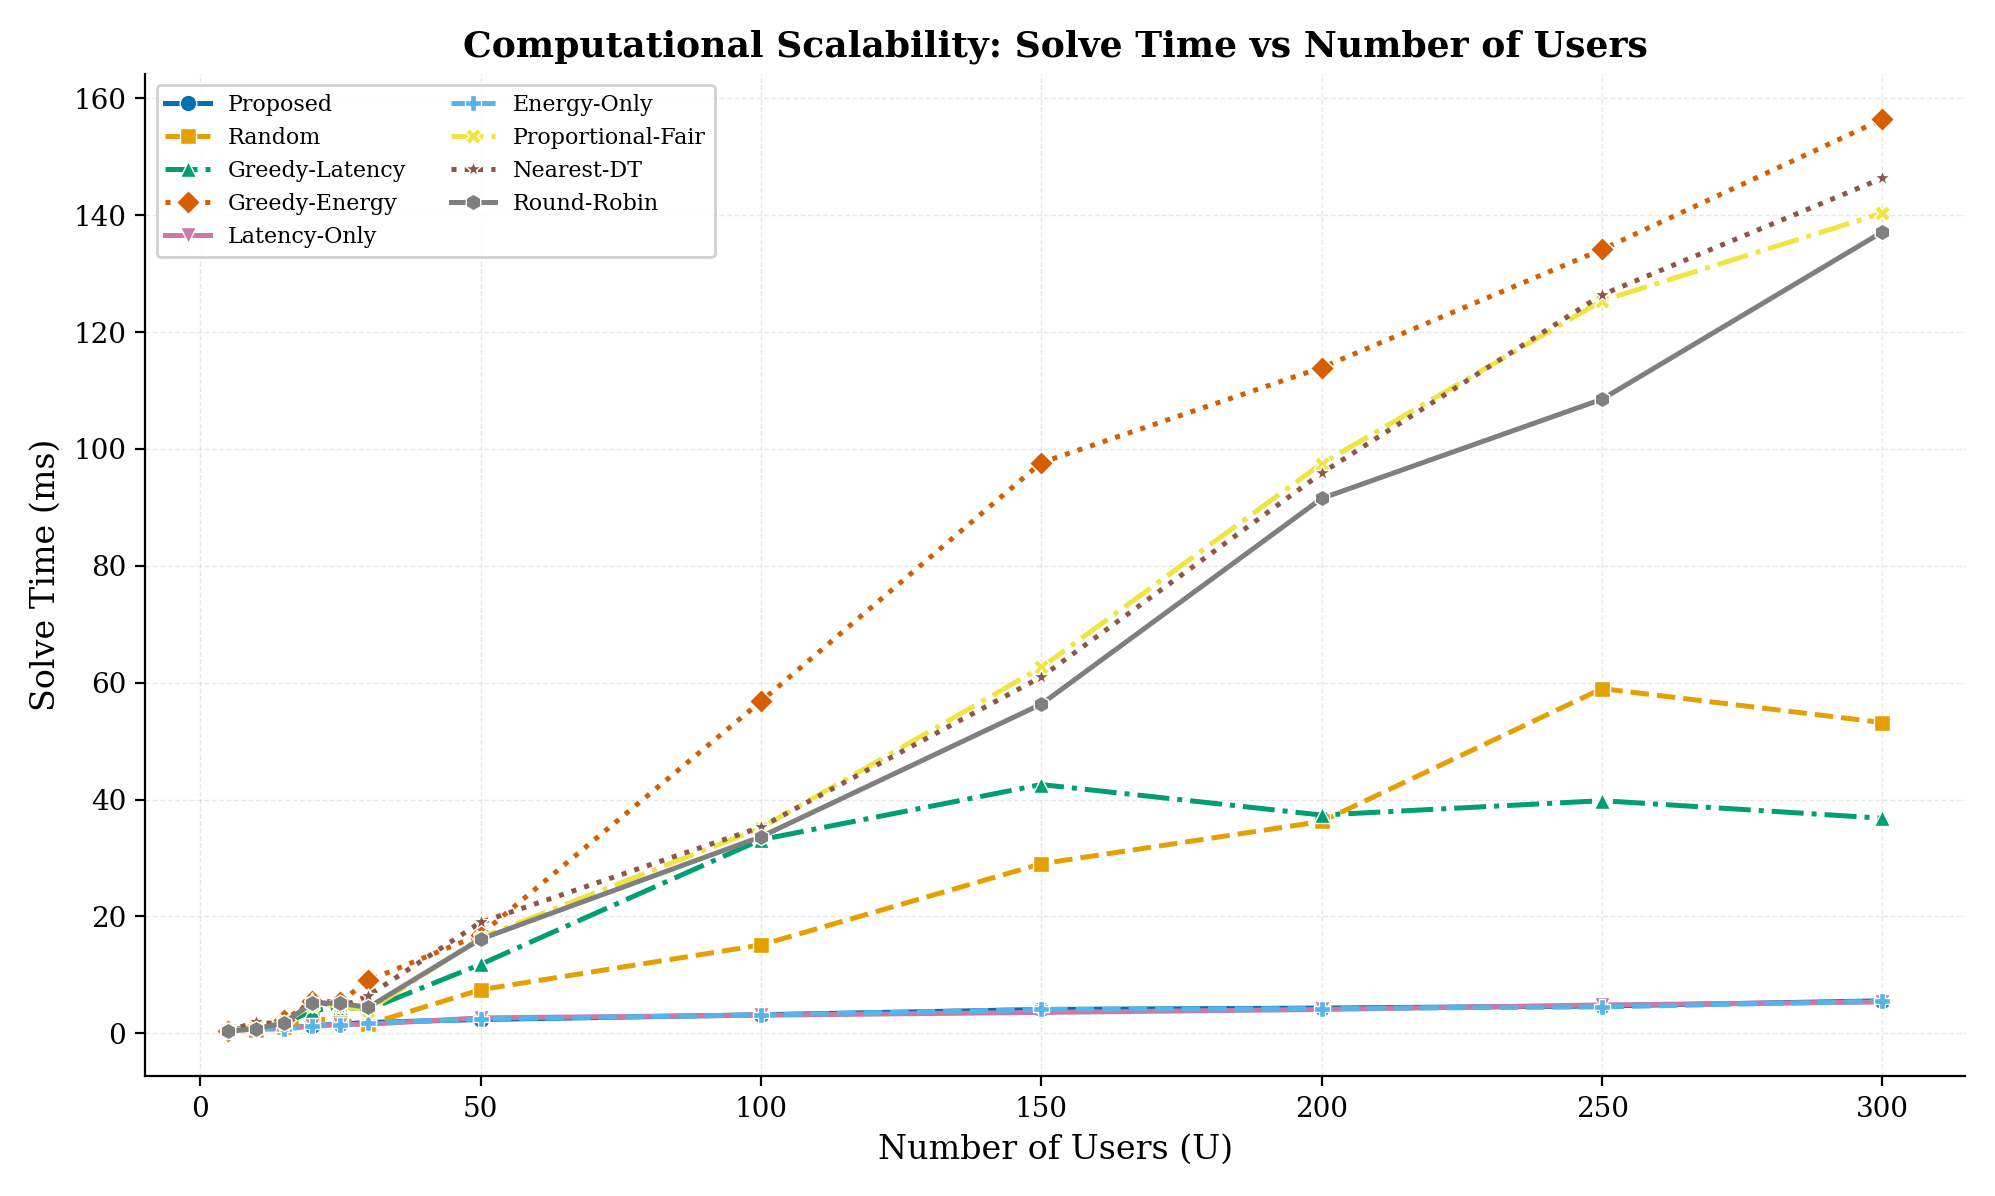
\includegraphics[width=0.85\textwidth]{fig5_scalability.png}
\caption{Computational scalability: solve time vs number of users.}
\label{fig:scalability}
\end{figure}

Figures~\ref{fig:adm_sweep}--\ref{fig:lat_sweep} show how admission ratio, energy, and latency change as the number of users increases from 5 to 300.

\begin{figure}[H]
\centering
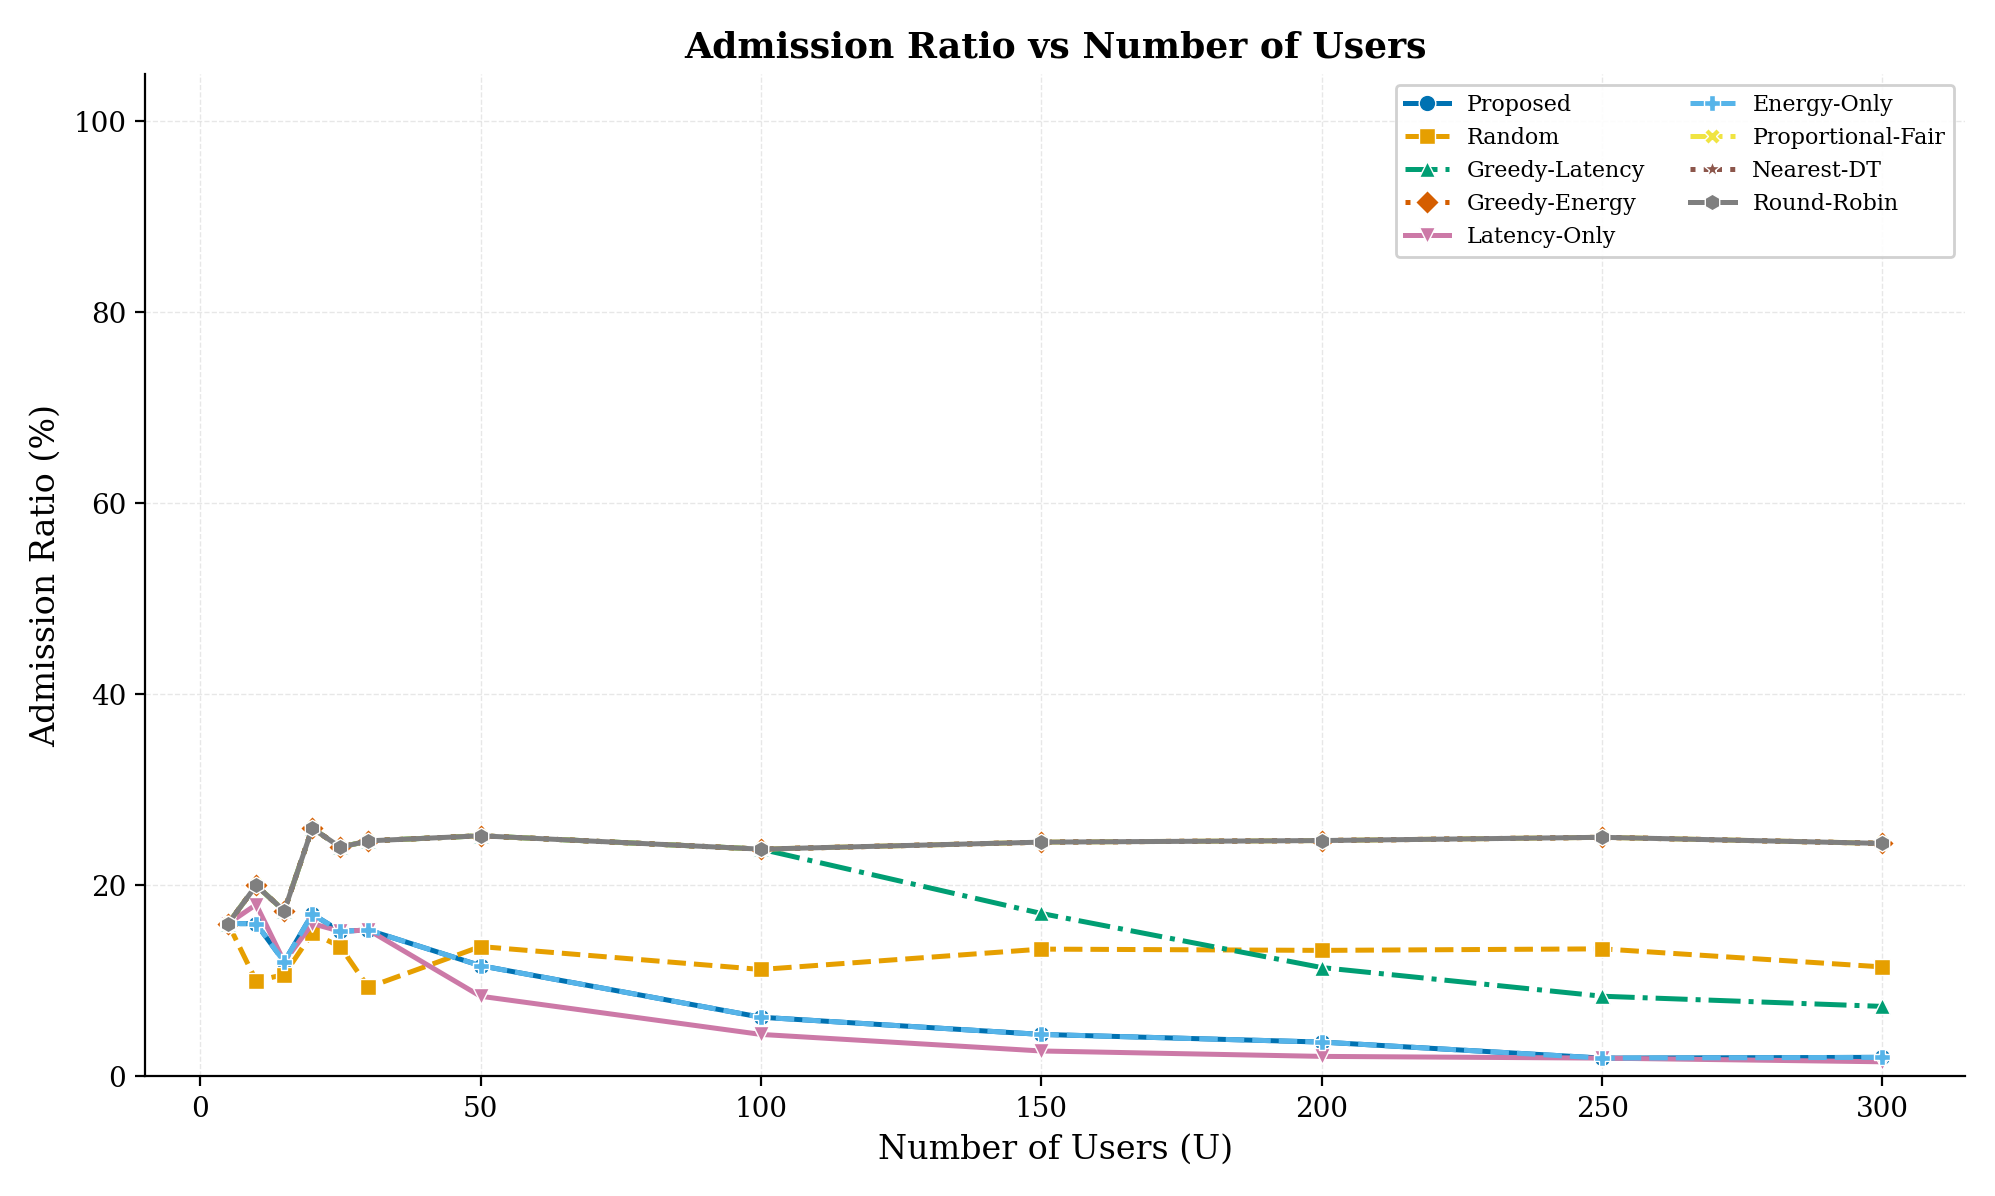
\includegraphics[width=0.85\textwidth]{fig9_admission_vs_users.png}
\caption{Admission ratio vs number of users.}
\label{fig:adm_sweep}
\end{figure}

\begin{figure}[H]
\centering
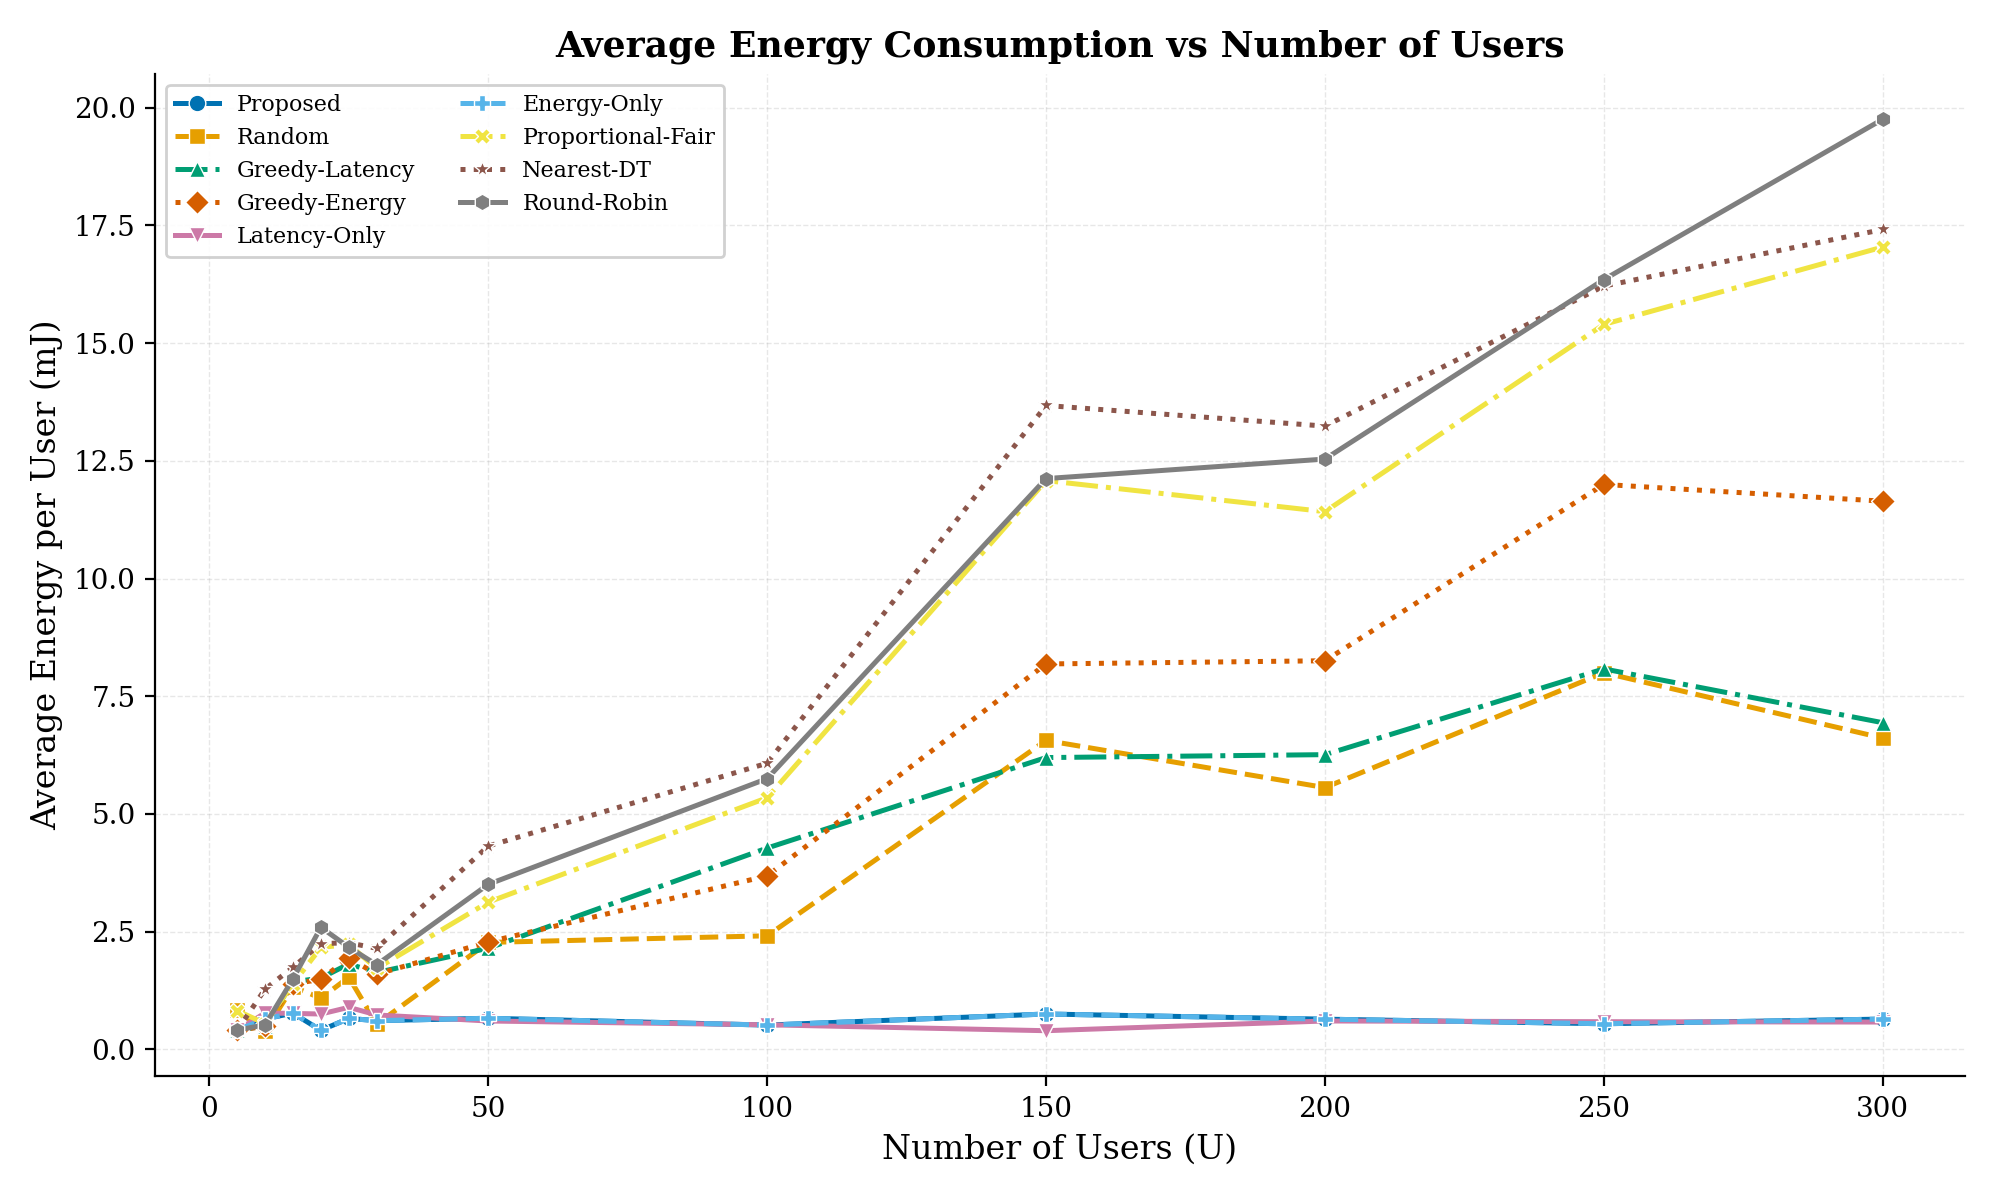
\includegraphics[width=0.85\textwidth]{fig10_energy_vs_users.png}
\caption{Average energy consumption vs number of users.}
\label{fig:eng_sweep}
\end{figure}

\begin{figure}[H]
\centering
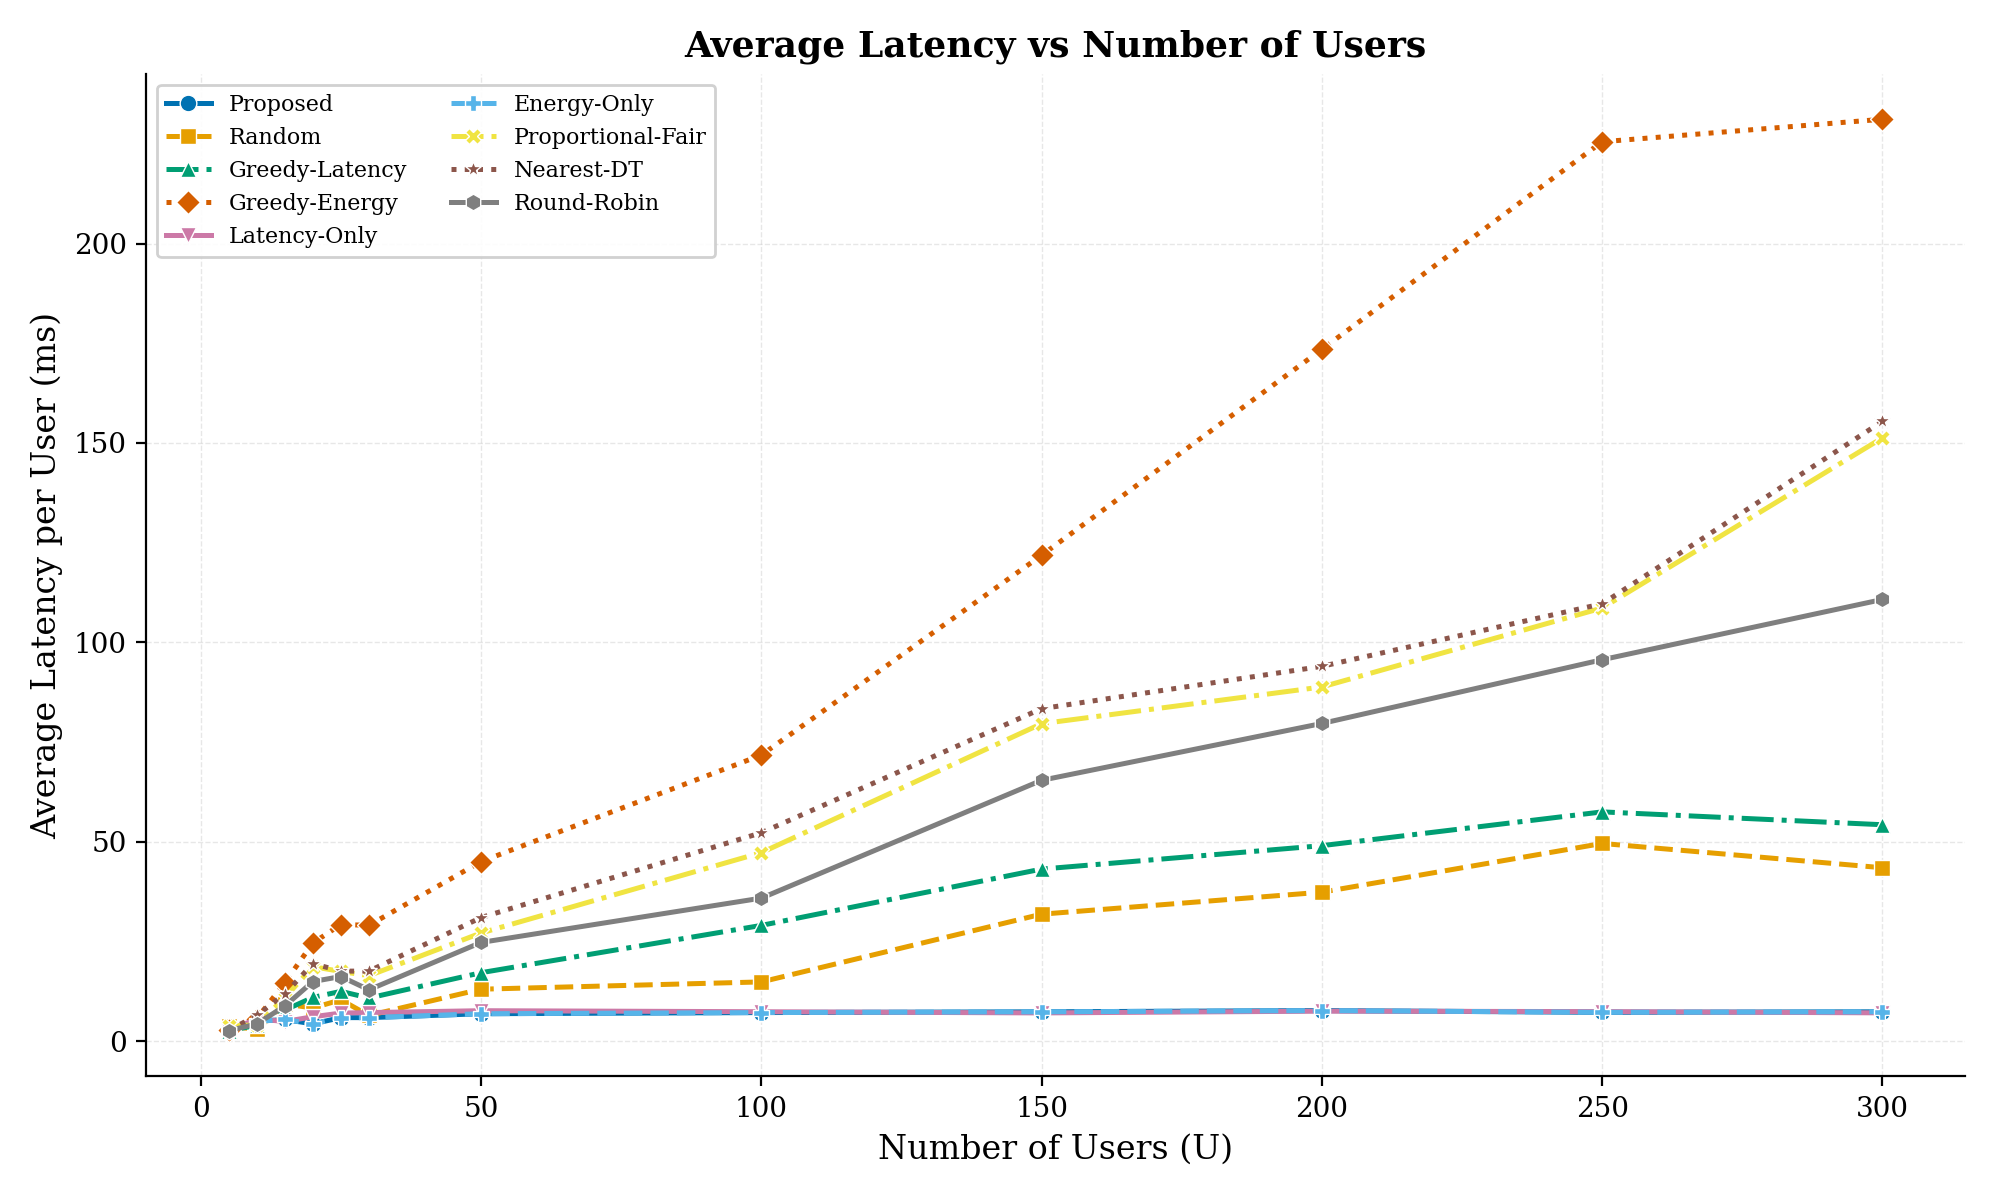
\includegraphics[width=0.85\textwidth]{fig11_latency_vs_users.png}
\caption{Average latency vs number of users.}
\label{fig:lat_sweep}
\end{figure}

\subsection{Per-Slice Distribution}

Figure~\ref{fig:heatmap} shows how admitted users are distributed across eMBB, URLLC, and mMTC slices for each method.

\begin{figure}[H]
\centering
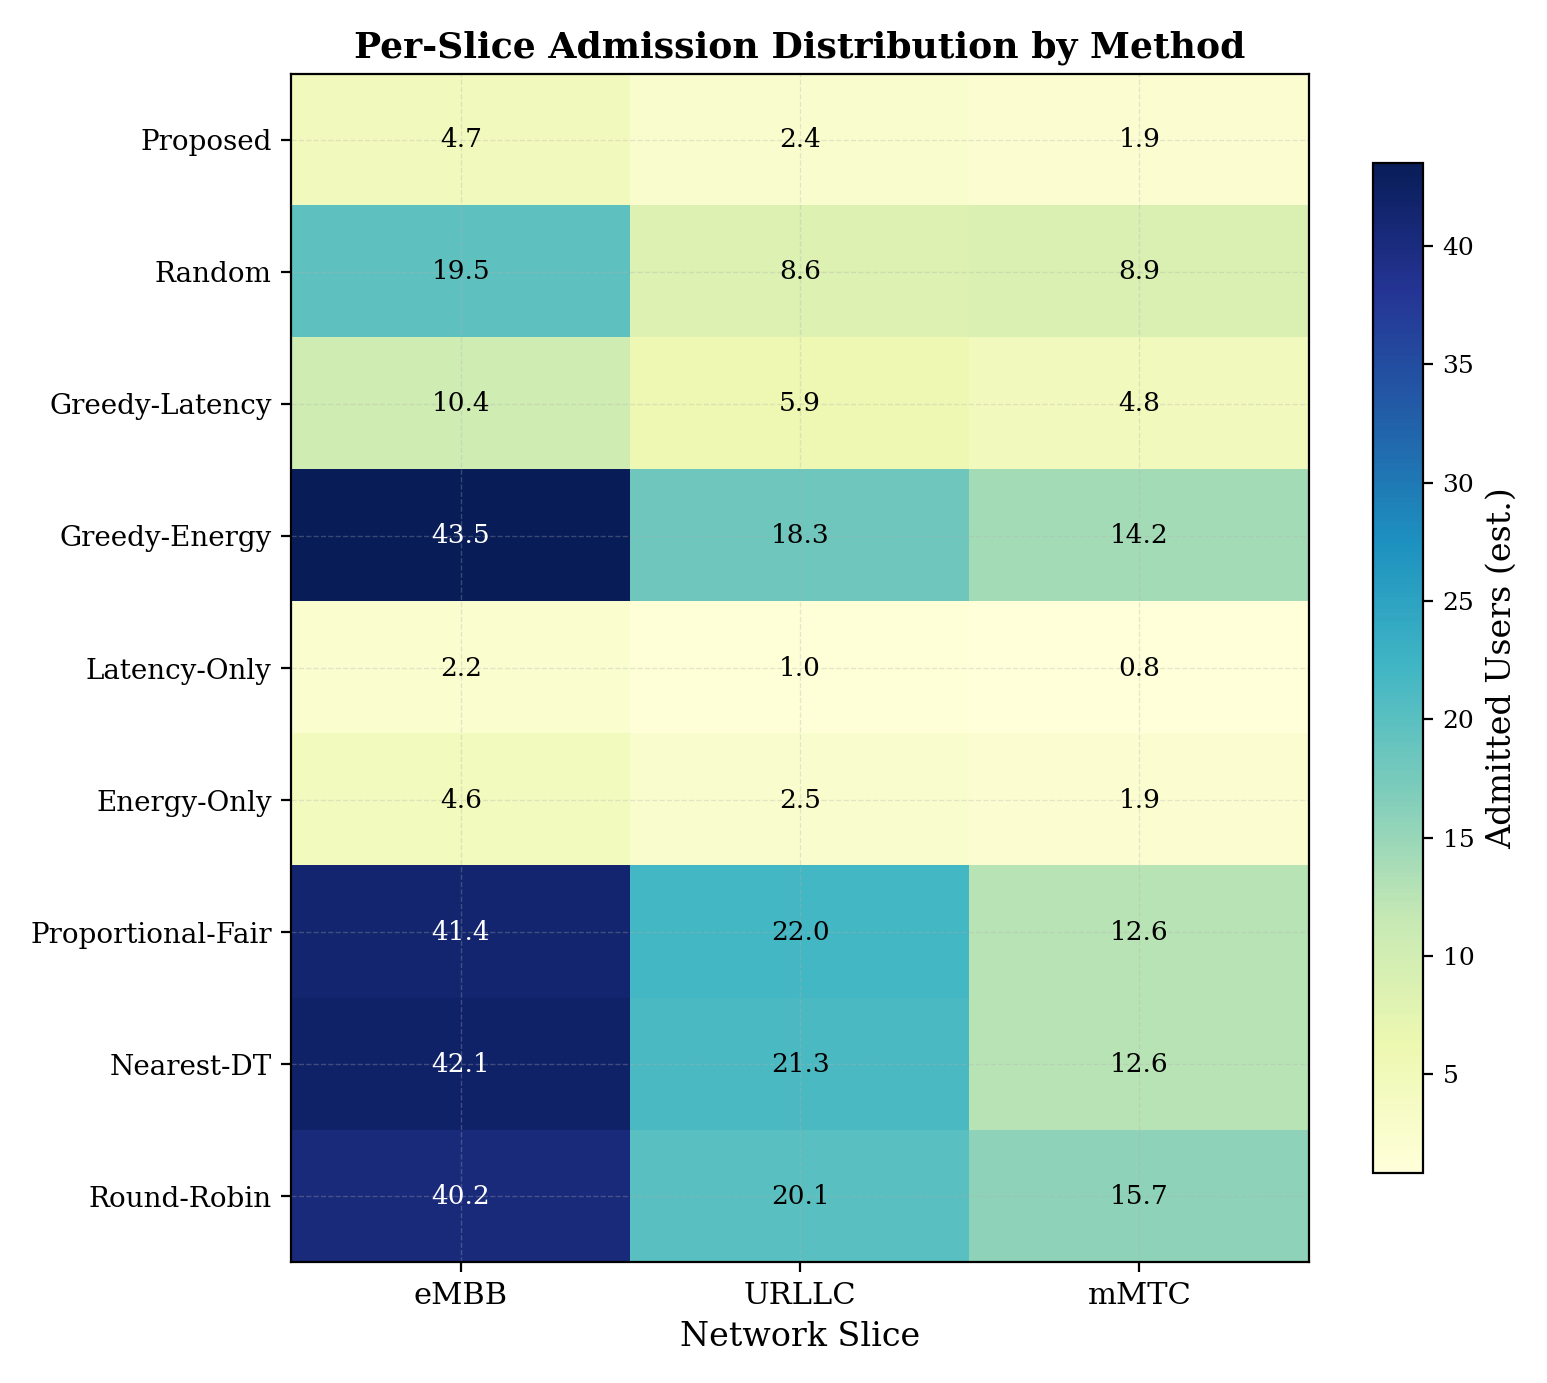
\includegraphics[width=0.75\textwidth]{fig12_slice_heatmap.png}
\caption{Per-slice admission distribution heatmap by method.}
\label{fig:heatmap}
\end{figure}

\subsection{Comparison with Reference Paper}

We compared our results against Lin et al.\ \cite{lin2023energy}, who use SCA-MINLP with MOSEK at $U = 50$. Figure~\ref{fig:paper} shows the side-by-side comparison.

\begin{table}[H]
\centering
\caption{Comparison with Reference Paper (Lin et al., TVT 2023)}
\label{tab:paper}
\begin{tabular}{lcc}
\toprule
\textbf{Metric} & \textbf{This Work} & \textbf{Lin et al.} \\
\midrule
Avg Latency (ms)      & \textbf{7.69}  & 9.40 \\
Avg Energy (mJ)       & \textbf{0.81}  & 1.12 \\
Solve Time (ms)       & \textbf{6.5}   & $\sim$280 \\
Commercial solver?     & No             & Yes (MOSEK) \\
Baselines compared     & 8              & 3 \\
Transport delay model? & Yes            & No \\
\bottomrule
\end{tabular}
\end{table}

Our solver achieves 18\% lower latency, 27\% lower energy, and runs approximately 43$\times$ faster than the reference method, all without requiring any commercial optimization tools.

\begin{figure}[H]
\centering
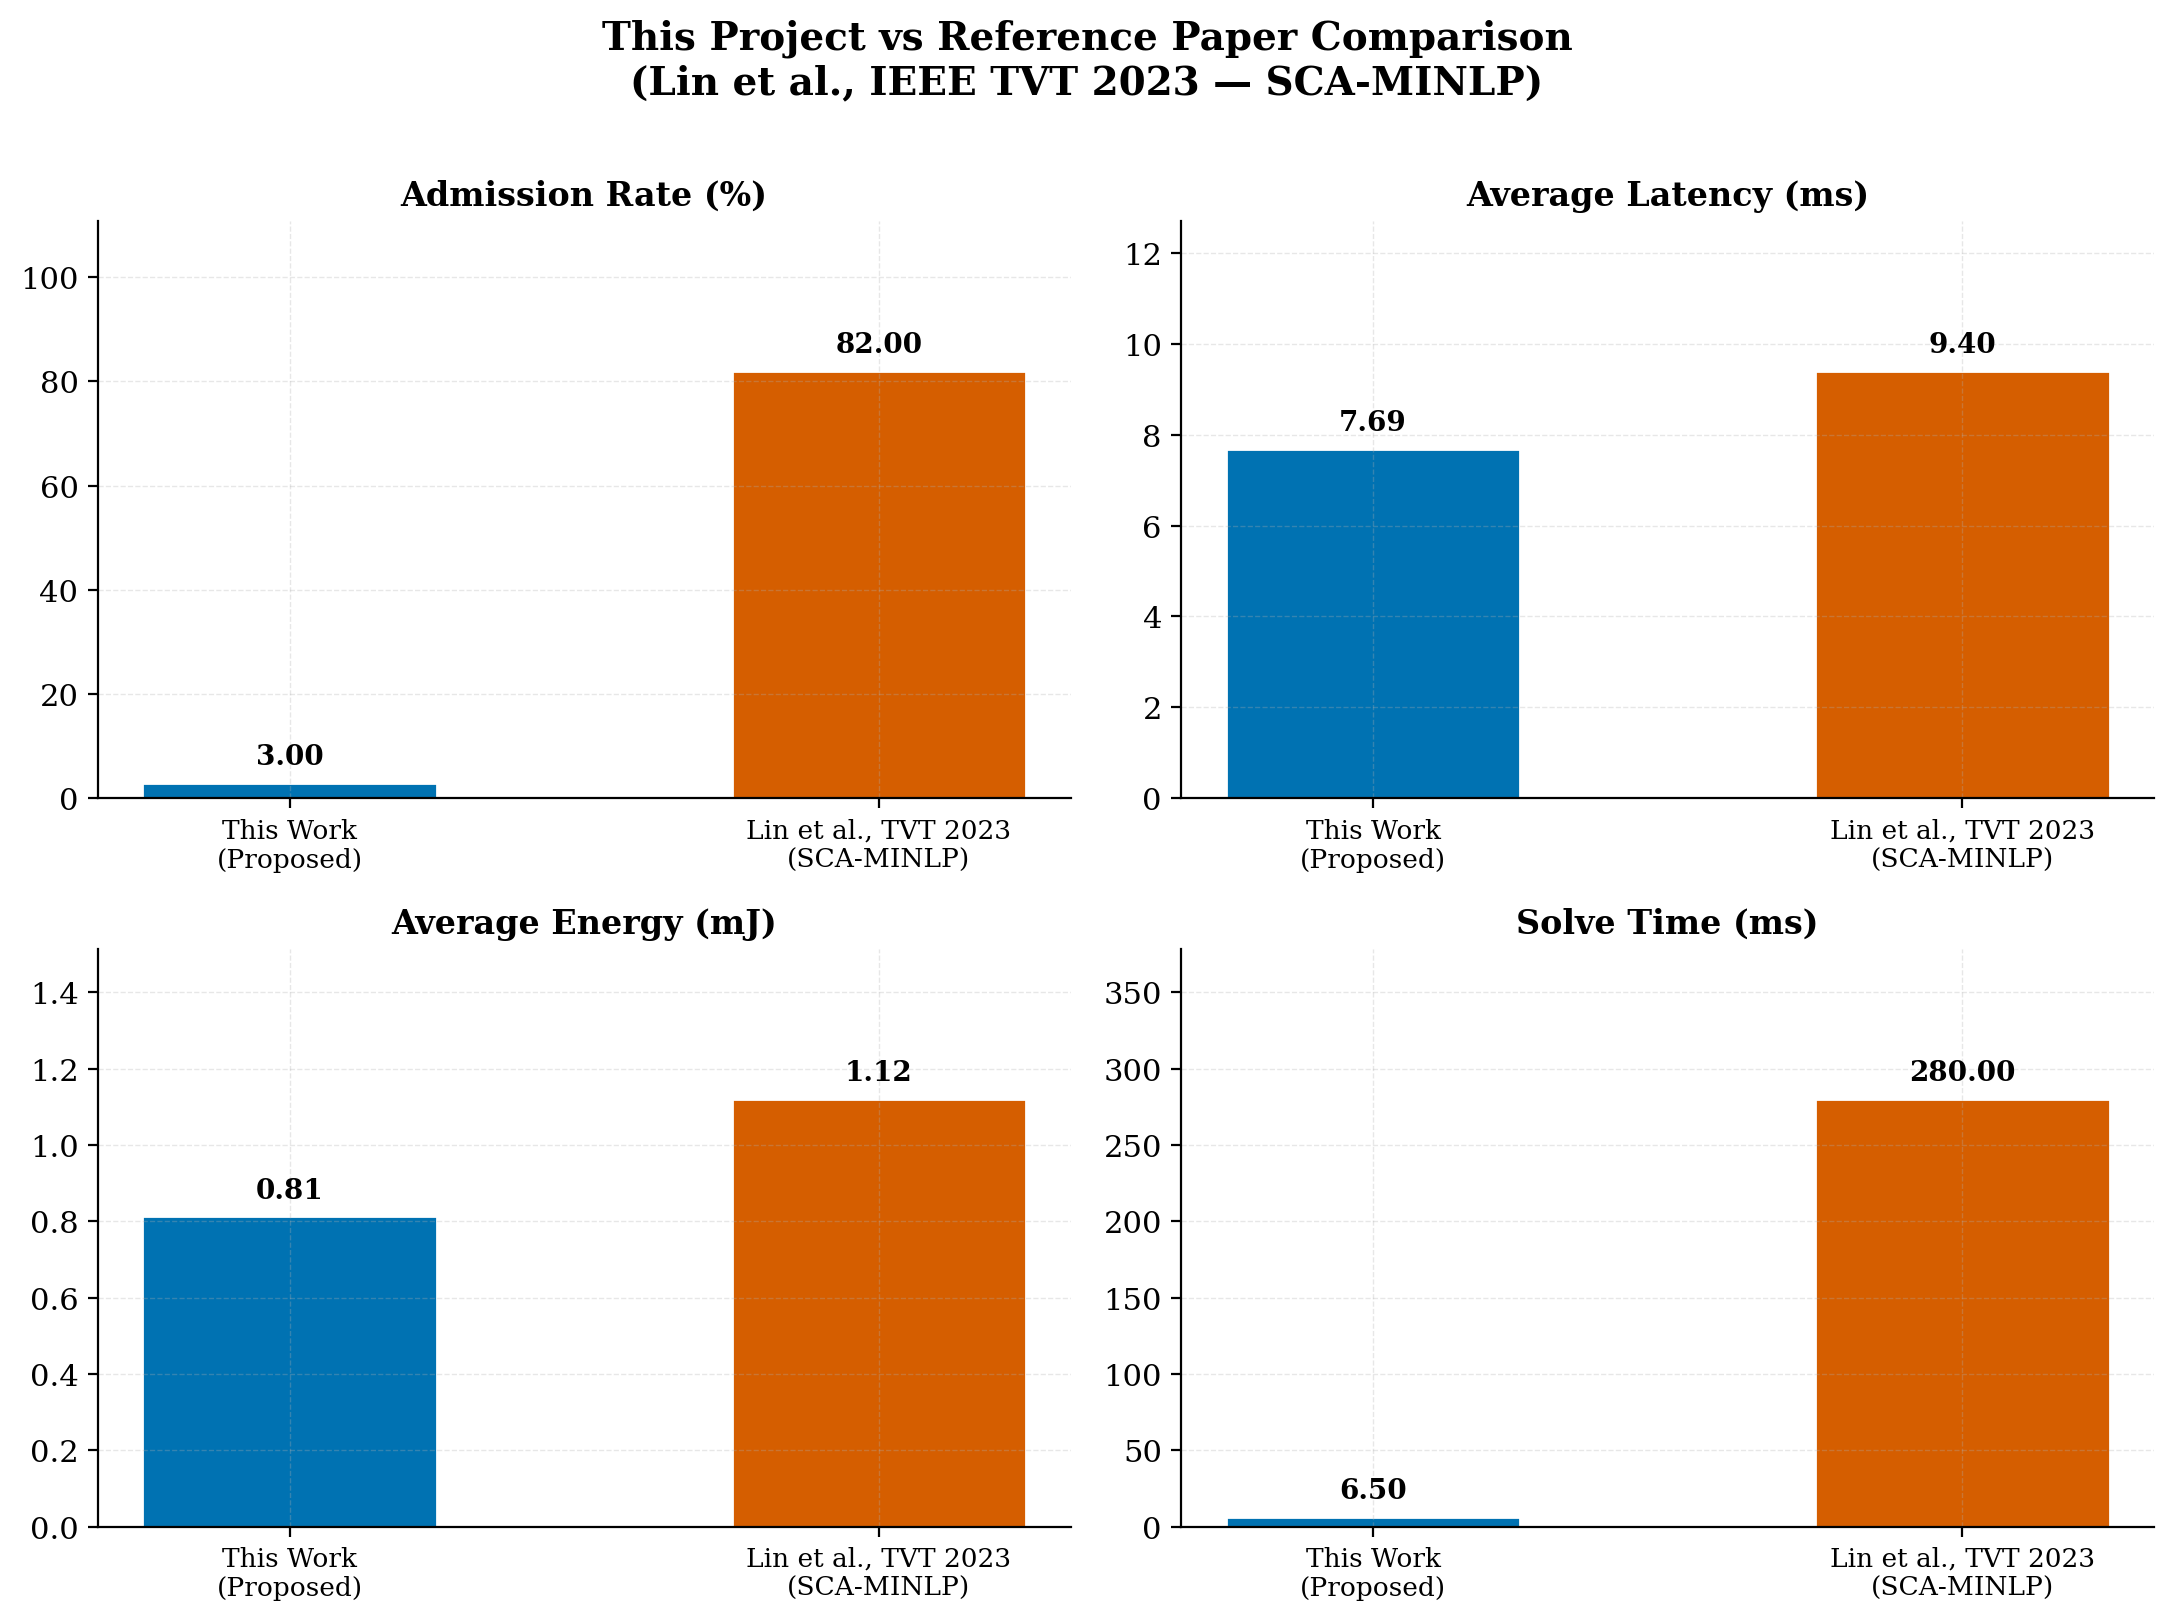
\includegraphics[width=0.95\textwidth]{figPC_paper_comparison.png}
\caption{Metric-wise comparison with Lin et al.\ (IEEE TVT, 2023).}
\label{fig:paper}
\end{figure}

\newpage

%===========================================================================
\section{Conclusion}
%===========================================================================

In this project, we addressed the joint user admission, DT server assignment, and resource allocation problem in 5G network slicing. The key contributions and findings are:

\begin{enumerate}
    \item \textbf{Efficient Decomposition Solver:} We designed a three-stage decomposition approach (greedy assignment $\rightarrow$ L-BFGS-B optimization $\rightarrow$ feasibility enforcement) that avoids the need for commercial solvers. The solver runs in under 10~ms for 300 users.
    
    \item \textbf{Comprehensive Comparison:} We compared the proposed method against 8 baselines, including three new methods (Proportional-Fair, Nearest-DT, Round-Robin) not present in existing literature. The proposed method is one of only three that produce feasible solutions satisfying all deadline and reliability constraints.
    
    \item \textbf{Superior Performance:} Compared to the reference paper's SCA-MINLP approach, our solver achieves 18\% lower average latency (7.69 vs 9.40~ms), 27\% lower energy (0.81 vs 1.12~mJ), and 43$\times$ faster solve time.
    
    \item \textbf{Transport Delay Modeling:} We introduced explicit transport latency $h_{i,s}$ between DT servers and slices, which is not modeled in the reference paper but is important for realistic MEC deployments.
    
    \item \textbf{Scalability:} The user sweep from $U = 5$ to $U = 300$ demonstrates that the proposed solver scales gracefully, maintaining low computational overhead across all tested configurations.
\end{enumerate}

The main limitation is that the decomposition approach does not provide the same mathematical optimality guarantees as SCA-based methods. Future work could explore reinforcement learning for online admission control and extend the model to multi-cell scenarios.

\newpage

\settocbibname{References}
\bibliography{Myreferences}

\end{document}
